% !TEX root = ../main.tex
\chapter{Resultats}
\label{chap:resultats}

Aquest capítol llegeix els artefactes del Capítol~\ref{chap:implementacio} sota el protocol del Capítol~\ref{chap:metodologia}. No es reobren el POSG, l'ablació ni el motor: aquí es mesura. Tres ancoratges es donen per fixats: \texttt{v12} és el millor resultat \emph{observat} a la matriu; \texttt{v14} és l'heurística de \emph{servei} (fulla, prior, executor i bot de \emph{ladder}), no el sostre de rendiment; MaskablePPO s'avalua fora de la matriu, contra \texttt{v12}.

Les fonts internes són els 784 CSV de \path{data/benchmarks/all_10k/gen9randombattle} ---\textbf{6.409.000} partides dirigides---, produïts pel pipeline de la Secció~\ref{sec:reporting_impl} (\texttt{generate\_heatmap.py}, \texttt{elo\_ranking.py}, informes a \path{src/p00_core/reporting/agents/}) i \path{src/p05_ppo_drl/RESULTS.md}. Un \textbf{resultat observat} és una taxa o un comptador; una \textbf{interpretació} relaciona indicadors amb el disseny; una \textbf{hipòtesi explicativa} requeriria una ablació nova per confirmar-se.

% ============================================================
\section{Protocol de lectura dels resultats}
\label{sec:res_protocol}

28 agents, cadascun com a \emph{nosaltres} contra 28 oponents, format \texttt{gen9randombattle}, estructurats segons la taxonomia de la Taula~\ref{tab:taxonomy}. Fitxers dirigits \texttt{A\_vs\_B.csv}. PPO es llegeix a part (Secció~\ref{sec:res_ppo}).

\begin{table}[H]
\centering
\caption{Taxonomia dels 28 agents del gauntlet \texttt{gen9randombattle}. Els identificadors es mantenen en anglès. El prefix de la figura de calor indica el paradigma: (H)~heurística, (MM)~minimax, (MCT)~MCTS, (IL)~imitació, (B)~baseline.}
\label{tab:taxonomy}
\small
\begin{tabular}{llp{8.2cm}}
\toprule
\textbf{IDs} & \textbf{Paradigma} & \textbf{Què és, en una frase} \\
\midrule
\texttt{random}, \texttt{max\_power}, \texttt{one\_step}, \texttt{safe\_one\_step}, \texttt{abyssal}, \texttt{simple\_heuristic}
  & Baselines (B)
  & Referents de \textit{poke-env} i d'estil Pokechamp: atzar, potència bruta, un pas de dany, i heurístiques de matchup. \\
\texttt{v1}--\texttt{v14}
  & Heurístiques (H)
  & Escala d'ablació per construcció: cada versió afegeix una peça de coneixement expert (dany, hazards, Tera, Yomi,\ldots). \\
\texttt{v15}--\texttt{v17}
  & Minimax 1-ply (MM)
  & Maximin analític d'un torn sobre \texttt{HeuristicV14}; sense \texttt{LocalSim}. \\
\texttt{v18}--\texttt{v20}
  & IS-MCTS (MCT)
  & 100 simulacions $\times$ 5 torns de \texttt{LocalSim}; cel·les amb $n=1.000$. \\
\texttt{v21}
  & IL híbrid (IL)
  & Macro XGBoost (mou vs canvia) + execució \texttt{v14}. \\
\texttt{v22}
  & IL pur (IL)
  & El mateix macro, dos XGBoost, \textbf{sense} \texttt{v14}. \\
\texttt{v23+}
  & PPO (fora del gauntlet)
  & Framework a \texttt{src/p05\_ppo\_drl/}; no forma part d'aquesta matriu. \\
\bottomrule
\end{tabular}
\end{table}


La fila és l'agent analitzat i la columna, l'oponent. Un 59,91 a la cel·la \texttt{v12} $\times$ Abyssal indica 5.991 victòries de 10.000 en aquell fitxer dirigit.

Cada cel·la és una proporció binomial. Els intervals són Wilson al 95\% (Equació~\ref{eq:wilson_ci}); els tres pisos mostrals són els de la Taula~\ref{tab:ci_n}. A $n=10.000$ el marge màxim d'una taxa individual és de $\pm 0{,}98$~pp; a $n=1.000$ (totes les cel·les MCTS), $\pm 3{,}10$~pp. La Pokédex no entra a $\mathrm{Var}(\hat p)$: s'estima una taxa marginal sota el generador d'equips de la Generació~IX.

Per a la comparació entre dues condicions o agents independents, s'aplica el contrast de dues proporcions (Equacions~\ref{eq:se_diff}--\ref{eq:ci_diff}): a $n=10.000$, la diferència mínima detectable per a una significança estadística al nivell $\alpha=0{,}05$ és de $|\Delta \hat{p}| \ge 1{,}39$~pp ($z \ge 1{,}96$, tercera columna de la Taula~\ref{tab:ci_n}); a $n=1.000$, el llindar és de $|\Delta \hat{p}| \ge 4{,}38$~pp. Les diferències inferiors a aquests llindars es troben dins el marge d'error conjunt i es consideren empats tècnics o variacions no significatives que no admeten interpretació de superioritat.

\begin{itemize}
    \item Fila no MCTS: \textbf{253.000} partides ($25\times 10.000$ i $3\times 1.000$ contra MCTS).
    \item Fila MCTS: \textbf{28.000} partides ($28\times 1.000$).
    \item Matriu: \textbf{6.409.000} partides dirigides. Les orientacions recíproques sumen $\approx 100\%$ i l'autojoc se situa prop del 50\%.
\end{itemize}

La taxa global d'una fila no MCTS pondera els oponents MCTS deu vegades menys; en una fila MCTS tots pesen igual. La comparació entre paradigmes es basa en cel·les comunes ---especialment contra \texttt{v12}---, no en una única ordenació global. Les proves de desenvolupament amb 100 partides no entren a les conclusions.

% ============================================================
\section{Controls globals de la matriu}
\label{sec:res_controls}

Abans d'interpretar versions concretes, es comproven la cobertura, la distribució de taxes i la durada de les batalles sobre les 784 cel·les dirigides:
\begin{itemize}
    \item \textbf{Cobertura:} La reducció mostral segueix estrictament el paradigma (10.000 partides per cel·la al bloc general i 1.000 a MCTS pel cost computacional de les simulacions), assegurant la consistència del banc d'avaluació.
    \item \textbf{Distribució de taxes:} La taxa de victòries es concentra al voltant del 50\% (autojoc i duels equilibrats) amb acumulacions als extrems (0\% i 100\%) degudes a referències febles (\texttt{random}, \texttt{max\_power}). Per aquest motiu, la taxa global no s'interpreta com una habilitat absoluta: millorar contra oponents febles té un valor discriminant molt limitat.
\end{itemize}

\begin{figure}[htbp]
    \centering
    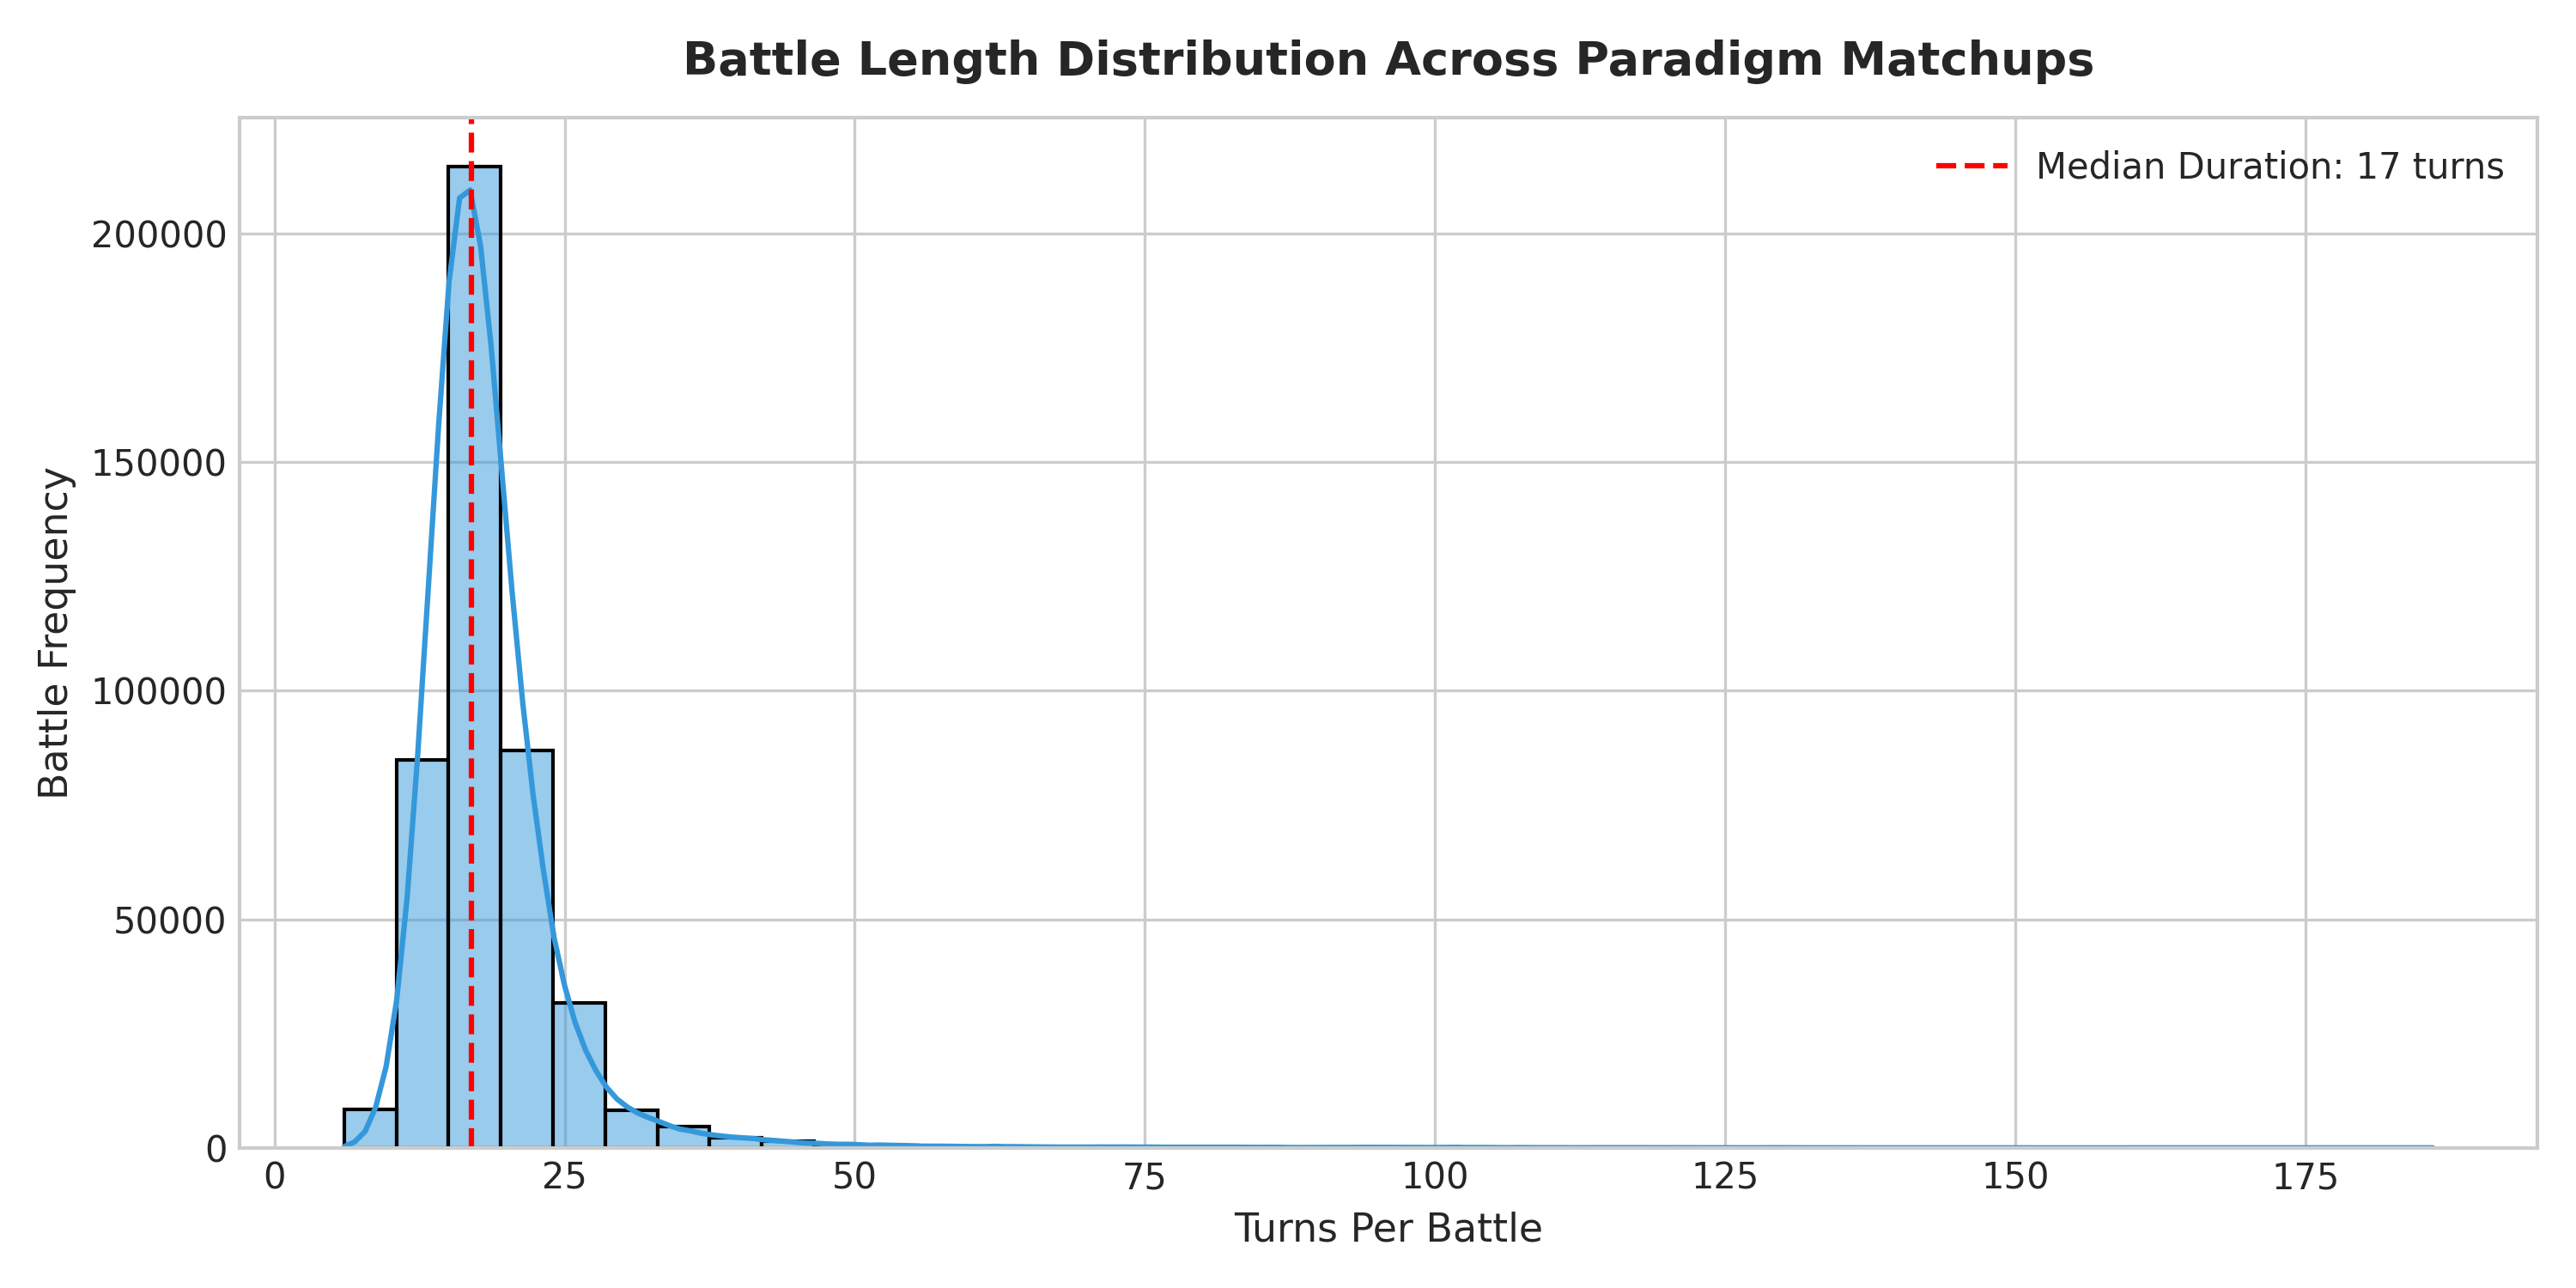
\includegraphics[width=0.88\linewidth]{images/results/game_length_distribution.png}
    \caption{Distribució de la durada de les batalles analitzades. La mediana és de 17 torns i hi ha una cua dreta de partides excepcionalment llargues.}
    \label{fig:length_distribution}
\end{figure}

Pel que fa a la durada (Figura~\ref{fig:length_distribution}), la mediana se situa clarament en 17 torns (amb el gruix entre 10 i 25 torns) i presenta una cua dreta per atrició defensiva o bucles de canvis. Com que dues polítiques poden assolir una mateixa taxa tancant ràpidament o bé dilatant el combat per conservació de recursos, les anàlisis posteriors combinen sempre torns, supervivents finals i motiu dels canvis.

% ============================================================
\section{Fil conductor de \texttt{v1} a \texttt{v22}}
\label{sec:version_timeline}

La Taula~\ref{tab:version_timeline} resumeix la seqüència abans d'analitzar-la. Les taxes globals són descriptives i no fan comparable l'MCTS amb la resta a causa de la ponderació diferent; la seva funció aquí és mostrar els canvis de règim.

\begin{table}[htbp]
\centering
\caption{Evolució de les preguntes i dels resultats entre \texttt{v1} i \texttt{v22}.}
\label{tab:version_timeline}
\small
\begin{tabularx}{\textwidth}{lXrX}
\toprule
\textbf{Versions} & \textbf{Pregunta que materialitzen} & \textbf{TV global} & \textbf{Patró observat} \\
\midrule
\texttt{v1}--\texttt{v6} & Fins on arriba refinar dany i ordre immediat? & 44--46\% & Altiplà; telemetria gairebé invariable. \\
\texttt{v7}, \texttt{v8}, \texttt{v10} & Què aporta valorar la posició i canviar? & 54--56\% & Salt a \texttt{v7}; afegits posteriors petits. \\
\texttt{v9}, \texttt{v11} & Preparació i perills només en torns segurs? & 59\% & Nou augment i aparició dels comptadors de ritme. \\
\texttt{v12} & Què aporten Tera i el substitut informat? & 69,01\% & Increment més gran i 59,91\% contra Abyssal. \\
\texttt{v13}, \texttt{v14} & Més inferència i model del rival sempre ajuden? & 67,63 / 62,03\% & Inversió: més complexitat, menys taxa global. \\
\texttt{v15}--\texttt{v17} & Un maximin d'un torn corregeix \texttt{v14}? & 53,80--57,89\% & La variant guiada discrepa menys i és la millor. \\
\texttt{v18}--\texttt{v20} & Cinc torns simulats superen l'horitzó curt? & 53,29--59,66\% & PUCT millora UCB1, però no supera \texttt{v12}. \\
\texttt{v21}, \texttt{v22} & Es pot imitar quan atacar o canviar? & 58,71 / 33,49\% & L'executor heurístic és determinant. \\
\bottomrule
\end{tabularx}
\end{table}

La primera meitat de la seqüència acumula coneixement explícit fins a \texttt{v12}. La segona canvia de paradigma, però la majoria de decisions encara passen per dreceres o priors derivats de \texttt{v14}. El patró general no és «algorisme més sofisticat, agent més fort», sinó «representació i coneixement adequats, seguits d'un mòdul que no els destrueixi».

PPO no rep un número \texttt{v23} ni forma part de la taula global. La seva pregunta és paral·lela: si una política neuronal inicialitzada amb \texttt{v8} pot arribar a \texttt{v12}. El resultat de 34,1\% contra aquest comparador es tracta a la Secció~\ref{sec:res_ppo}.

% ============================================================
\section{L'escala heurística: tres canvis de règim}
\label{sec:res_heur}

\begin{table}[H]
\centering
\caption[Seqüència heurística \texttt{v1}--\texttt{v14}.]{Seqüència heurística \texttt{v1}--\texttt{v14} (253.000 partides per fila). La taxa global no creix de manera monotònica: els increments principals apareixen a \texttt{v7}, \texttt{v9} i \texttt{v12}, i les dues versions posteriors disminueixen.}
\label{tab:heur_ladder}
\small
\begin{tabularx}{\textwidth}{llrr>{\raggedright\arraybackslash}X}
\toprule
\textbf{Agent} & \textbf{Règim} & \textbf{TV (\%)} & \textbf{contra Abyssal} & \textbf{Incorporació principal} \\
\midrule
\texttt{v1}--\texttt{v6} & Altiplà & 44,25--45,86 & 30,6--32,5 & Dany, clima, modificadors i canvis simples \\
\texttt{v7} & Posicional & 54,25 & 40,80 & Dany modificat i canvi segons l'enfrontament \\
\texttt{v8} & Posicional & 55,43 & 42,30 & Objectes, habilitats, pantalles, Trick Room \\
\texttt{v9} & Ritme segur & 58,86 & 46,64 & Perills i preparació \emph{només en torns lliures} \\
\texttt{v10} & Posicional & 55,66 & 41,86 & Status, sacrifici $\le 20\%$ HP, U-turn \\
\texttt{v11} & Ritme segur & 59,26 & 47,50 & Combinació de \texttt{v9} i \texttt{v10} \\
\texttt{v12} & Mecànica Gen.~IX & \textbf{69,01} & \textbf{59,91} & Tera i selecció del substitut \\
\texttt{v13} & Moviments revelats & 67,63 & 55,34 & Enfrontament amb moviments revelats i Tera conservador \\
\texttt{v14} & Model de rival & 62,03 & 51,36 & Perfil, sondeig inicial, rang de dany i final d'un torn \\
\bottomrule
\end{tabularx}
\end{table}


La Taula~\ref{tab:heur_ladder} i la Figura~\ref{fig:heur_overall_wr} sintetitzen l'evolució de la taxa de victòries global al llarg de la seqüència heurística \texttt{v1}--\texttt{v14}.

\begin{figure}[htbp]
    \centering
    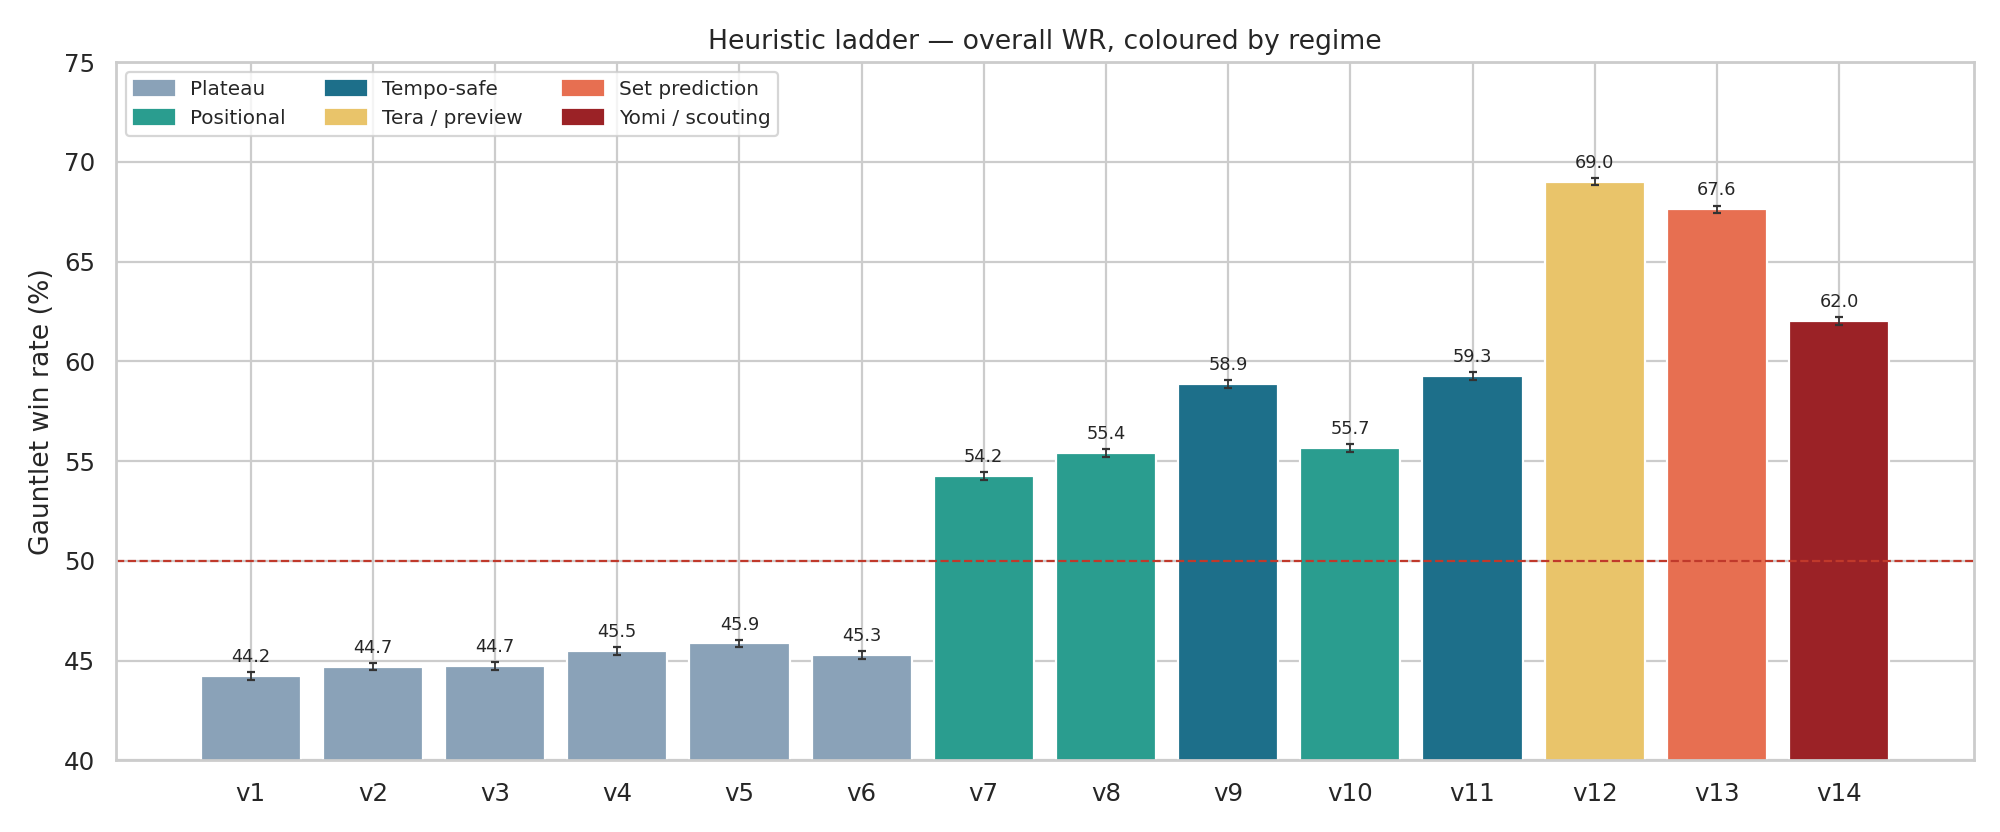
\includegraphics[width=0.95\linewidth]{images/heuristics/heur_overall_wr.png}
    \caption{Taxa global de victòries de \texttt{v1}--\texttt{v14} (253.000 partides per fila; les tres cel·les contra MCTS tenen $n=1.000$). S'observen canvis destacats a \texttt{v7}, \texttt{v9} i \texttt{v12}, seguits d'una disminució a \texttt{v13} i \texttt{v14}.}
    \label{fig:heur_overall_wr}
\end{figure}

\subsection{Altiplà \texttt{v1}--\texttt{v6}: rendiments decreixents del càlcul de dany}

La taxa global recorre \textbf{1,61~pp} (44,25--45,86\%). Els enfrontaments interns se situen prop del 50\%, mentre que contra Abyssal obtenen entre el 30,6\% i el 32,5\%.

En aquestes versions, afinar la fórmula de dany després d'incorporar efectivitat i STAB mostra rendiments decreixents. Els increments posteriors apareixen quan s'afegeixen decisions posicionals i recursos específics del format.

En el conjunt de la matriu (253.000 partides per fila; mitjanes ponderades per nombre de partides), registren aproximadament 1,02 canvis voluntaris per partida, cap Teracristal·lització i uns 4,6 recursos de reserva. Aquest perfil correspon a una política principalment ofensiva amb poca gestió posicional.

\subsection{Primer salt: \texttt{v7} (i \texttt{v8}/\texttt{v10})}

\texttt{v7} incorpora dany amb modificadors i canvis segons l'enfrontament. La taxa global passa d'aproximadament 45,5\% a \textbf{54,25\%}; contra Abyssal, d'aproximadament 32\% a \textbf{40,8\%}.

\texttt{v8} (KO de prioritat conservador i immunitats d'habilitat ja revelades) afegeix 1,2~pp. \texttt{v10} (estats, sacrificis i moviments de pivot) obté una taxa similar a \texttt{v8} (55,66\% i 55,43\%).

La telemetria també canvia: els canvis voluntaris pugen a 1,47 per partida, \texttt{matchup\_switches} arriba a 0,41 i les accions de reserva baixen d'aproximadament 4,6 a 2,18. L'agent passa a seleccionar canvis de manera explícita.

Els perills d'entrada i els moviments de preparació s'incorporen a \texttt{v9}; els comptadors \texttt{setup\_uses} i \texttt{hazard\_sets} deixen de ser zero.

\subsection{Segon salt: \texttt{v9} / \texttt{v11}}

Amb \texttt{v9}, els perills d'entrada i els moviments de preparació només s'utilitzen quan l'agent és més ràpid i resisteix l'STAB rival. La taxa global puja a \textbf{58,86\%} i el resultat contra Abyssal a \textbf{46,64\%}. \texttt{v11} combina aquest bloc amb \texttt{v10} i afegeix 0,4~pp; la contribució addicional és petita en aquesta matriu.

\texttt{v9}/\texttt{v11} són els primers amb aproximadament 1,6 moviments de preparació i 0,16 perills d'entrada per partida.

\subsection{Tercer salt: \texttt{v12}}

\texttt{v12} combina la Teracristal·lització i la selecció informada del substitut després d'un debilitament. La taxa global assoleix el \textbf{69,01\%}, suposant el major increment de tota la seqüència ($+9{,}75$~pp respecte al $59{,}26\%$ de \texttt{v11}). És, a més, el primer agent intern que supera amb claredat Abyssal i Simple Heuristic: \textbf{59,91\%} i \textbf{59,75\%}, respectivament ($n=10.000$, tal com s'il·lustra a la Figura~\ref{fig:heur_vs_baselines} enfront dels comparadors discriminants).

En la telemetria de matriu (recollida en l'empremta tàctica de la Figura~\ref{fig:heur_fingerprint}), utilitza la Teracristal·lització \textbf{0,96 vegades per partida}, registra només \textbf{0,01} accions de reserva i conserva \textbf{1,84} Pokémon, davant d'1,44 a \texttt{v11}. El canvi de comportament és substancial.

Tot i que totes dues millores s'introdueixen conjuntament en aquesta versió, la telemetria granular de la matriu permet desacoblar observacionalment la contribució relativa de cada mecanisme:
\begin{enumerate}
    \item \textbf{Impacte de la selecció del substitut (eliminació de \emph{fallbacks}):} A les versions prèvies (\texttt{v1}--\texttt{v11}), la manca d'un gestor per als torns forçats per debilitament feia que l'agent invoqués el mecanisme per defecte (\texttt{fallback\_moves\_us}), seleccionant el substitut d'entrada uniformement a l'atzar. A \texttt{v12}, la resolució per aparellament (\texttt{\_get\_best\_switch}) redueix les accions de reserva de $\sim 3{,}5$ a pràcticament zero ($0{,}01$ per partida), evitant que l'agent regali la iniciativa entrant en desavantatge elemental greu.
    \item \textbf{Impacte de la Teracristal·lització (el contrast natural amb \texttt{v13}):} A la versió immediatament posterior (\texttt{v13}), la selecció informada del substitut es manté intacta, però l'ús de la Teracristal·lització es restringeix dràsticament, caient un \textbf{79\%} (de $0{,}96$ usos per partida a \texttt{v12} a només $0{,}20$ a \texttt{v13}). Malgrat aquesta reducció massiva de la Tera, el rendiment global només retrocedeix $\approx 1{,}4$~pp (de $69{,}01\%$ a $67{,}63\%$), el duel directe entre totes dues queda en empat virtual ($50{,}65\%$ vs $48{,}85\%$, separat per només $1{,}8$~pp, Taula~\ref{tab:heur_h2h}; el test de proporció respecte al 50\% d'equilibri llança $z = 1{,}30$, $p = 0{,}19$ per a \texttt{v12}, confirmant que la desviació respecte a la paritat és estadísticament no significativa) i \texttt{v13} fins i tot supera \texttt{v12} enfront de la cerca i la imitació (Taula~\ref{tab:v13_vs_search}).
\end{enumerate}

Aquest contrast observacional suggereix com a hipòtesi que el gruix principal del salt ($\approx 7$--$8$~pp) s'atribueix a l'eliminació dels canvis forçats atzarosos i a l'estabilització del posicionament tàctic, mentre que la Teracristal·lització afegeix un marge incremental d'aproximadament $\approx 1{,}4$~pp gràcies a la bonificació de dany elemental i la flexibilitat defensiva.

\begin{figure}[htbp]
    \centering
    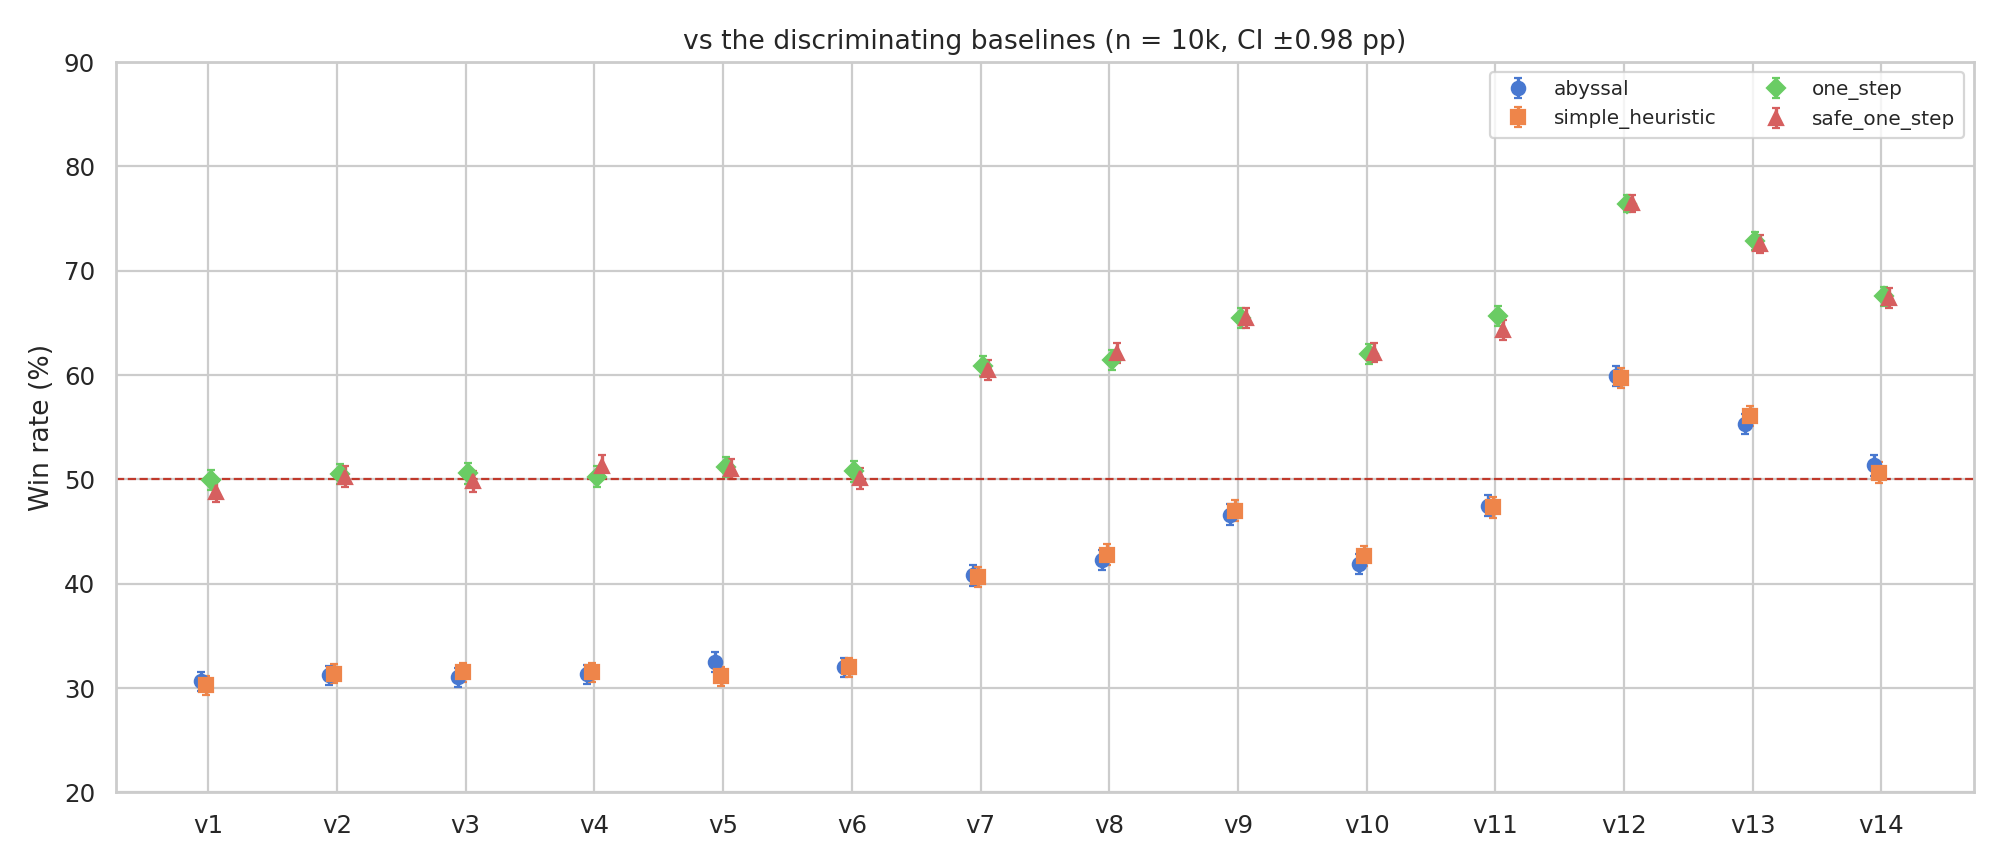
\includegraphics[width=0.95\linewidth]{images/heuristics/heur_vs_baselines.png}
    \caption{\texttt{v1}--\texttt{v14} contra els quatre agents de referència discriminants ($n=10.000$ per cel·la): Abyssal, Simple Heuristic, \texttt{one\_step} i \texttt{safe\_one\_step}. \texttt{v12} és el primer que deixa Abyssal i Simple Heuristic clarament per sota del 50\%. Random i MaxBasePower s'ometen: contra Random totes les heurístiques arriben al 97--98\% i la columna no discrimina.}
    \label{fig:heur_vs_baselines}
\end{figure}

\begin{figure}[htbp]
    \centering
    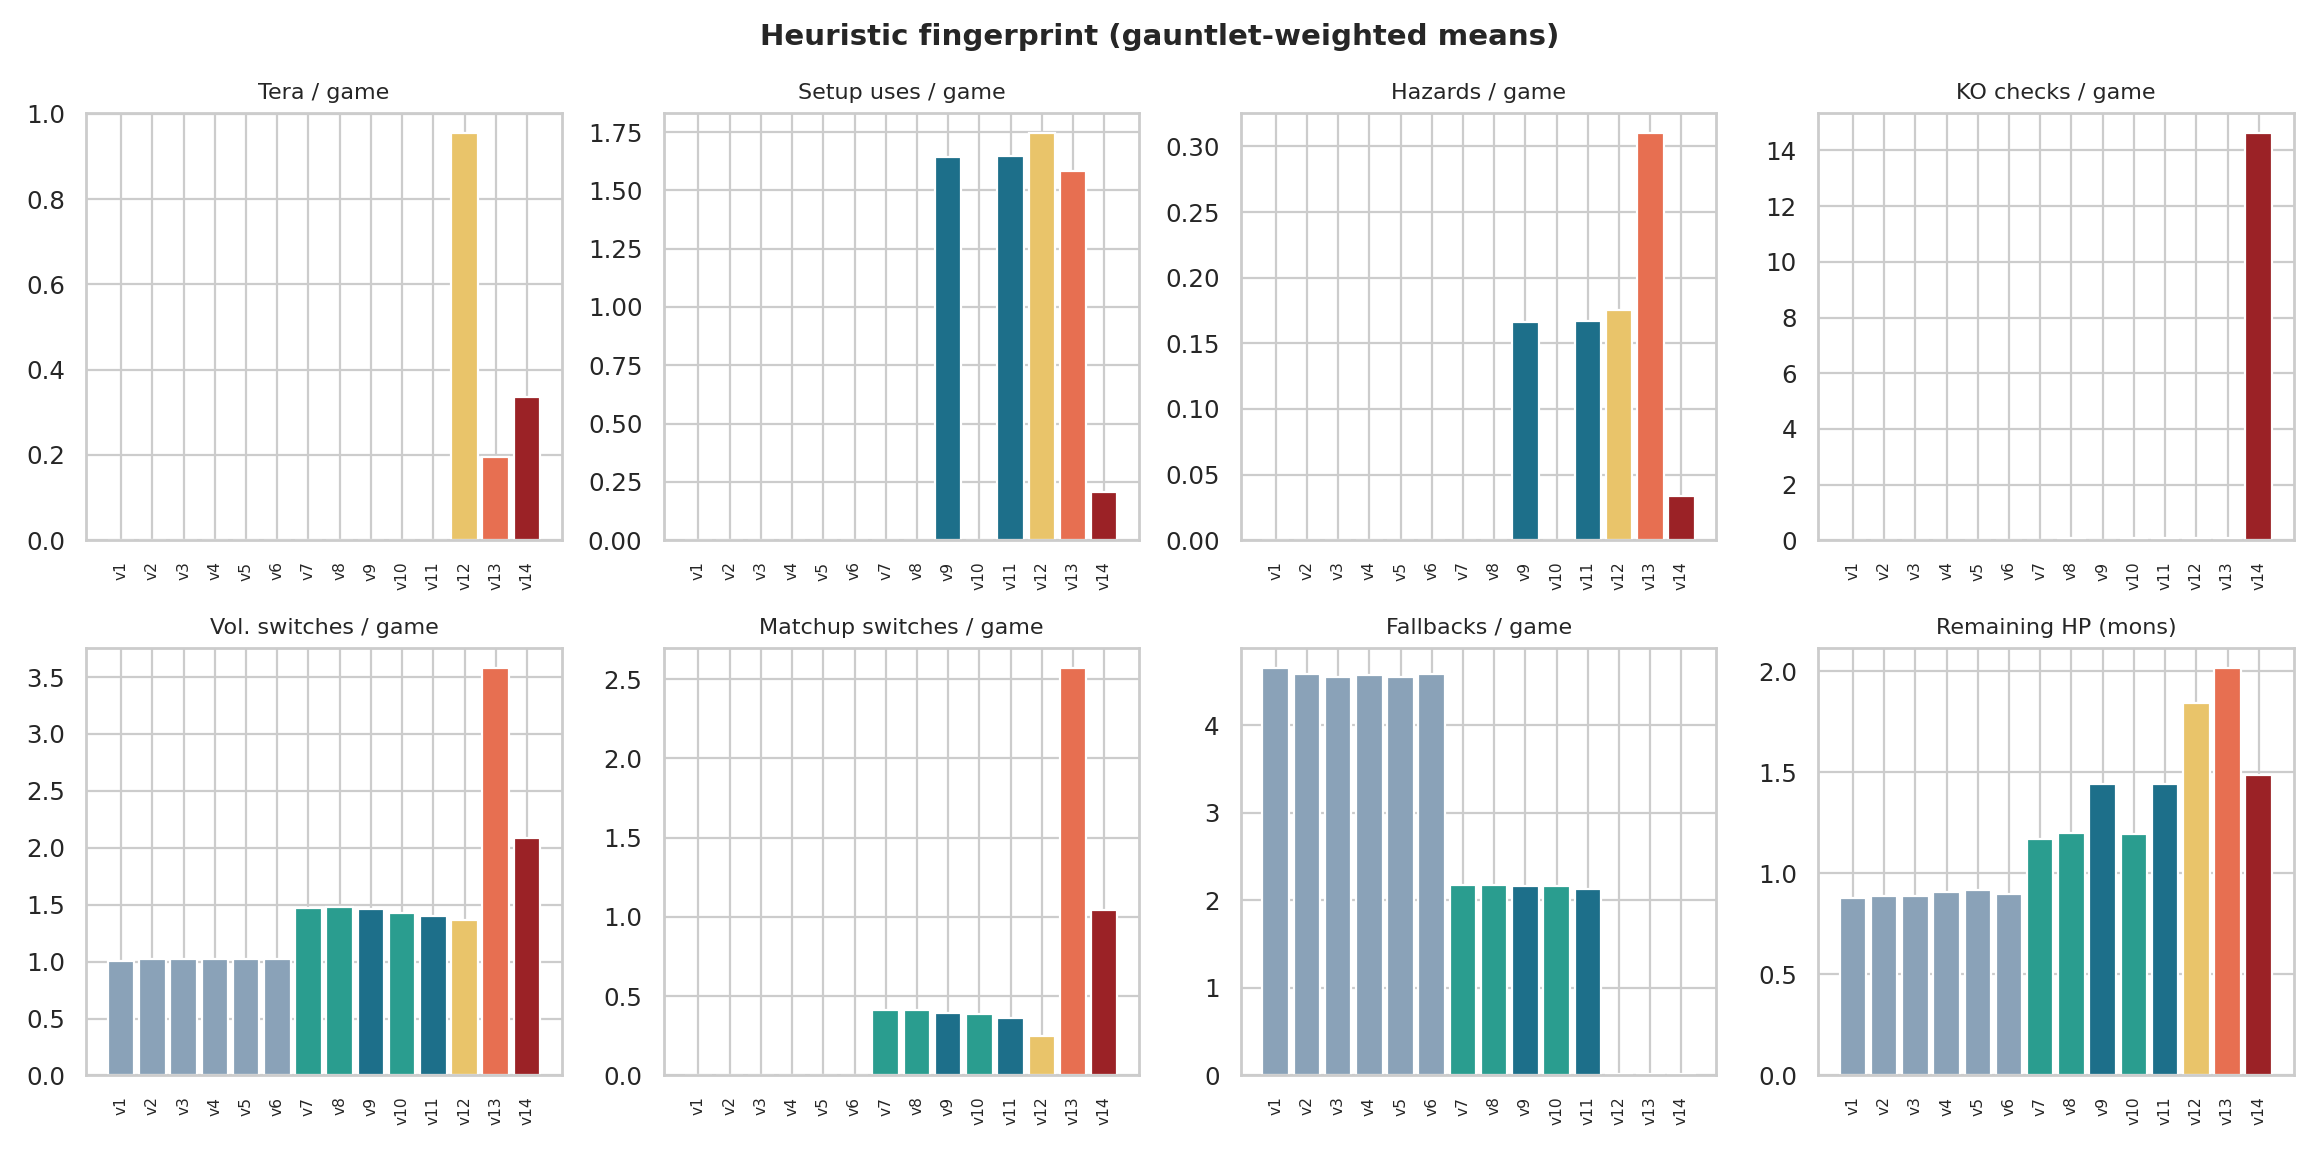
\includegraphics[width=0.95\linewidth]{images/heuristics/heur_fingerprint_bars.png}
    \caption{Empremta tàctica de la seqüència heurística (mitjanes ponderades de la matriu). \texttt{v12} utilitza la Teracristal·lització gairebé una vegada per partida; \texttt{v13}, 0,20 vegades. \texttt{ko\_checks} augmenta fins a aproximadament 15 a \texttt{v14}; la preparació i els perills d'entrada apareixen a partir de \texttt{v9}.}
    \label{fig:heur_fingerprint}
\end{figure}

% ============================================================
\FloatBarrier
\section{La inversió entre \texttt{v12}, \texttt{v13} i \texttt{v14}}
\label{sec:res_inversion}

La complexitat creix de \texttt{v12} a \texttt{v14}, però la taxa global observada disminueix. Aquest resultat mostra que l'herència de funcionalitats no implica una millora monotònica.

\begin{table}[H]
\centering
\caption{Cara a cara de la inversió, $n=10.000$ partides independents cada sentit. \texttt{v12} vs \texttt{v13} és un llançament de moneda (buit de 1,8~pp, cada IC $\pm 0{,}98$). \texttt{v14} perd clarament contra tots dos. Les sumes recíproques $\approx 100\%$ descarten un artefacte de seient.}
\label{tab:heur_h2h}
\small
\begin{tabular}{lrrr}
\toprule
\textbf{Fitxer} & \textbf{WR (\%)} & \textbf{Recíproc (\%)} & \textbf{Suma} \\
\midrule
\texttt{v12\_vs\_v13} & 50,65 & 48,85 & 99,50 \\
\texttt{v12\_vs\_v14} & 56,01 & 44,74 & 100,75 \\
\texttt{v13\_vs\_v14} & 57,71 & 41,60 & 99,31 \\
\bottomrule
\end{tabular}
\end{table}


Tal com reflecteix la Taula~\ref{tab:heur_h2h}, les dues orientacions de \texttt{v12} i \texttt{v13} difereixen només en 1,8~pp (50,65\% i 48,85\%) i no aporten una separació concloent (enfront de la paritat del 50\%, $z = 1{,}30$, $p = 0{,}19$ a l'orientació directa i $z = 2{,}30$, $p = 0{,}02$ a la recíproca; la taxa combinada de les 20.000 partides és del 50,90\%, situant la desviació en un marge pràcticament negligible de $<1$~pp). En canvi, \texttt{v14} queda clarament per sota de tots dos en els enfrontaments directes de manera estadísticament inequívoca (44,74\% davant \texttt{v12}, $z = 10{,}52$, $p < 10^{-15}$, i 41,60\% davant \texttt{v13}, $z = 16{,}80$, $p < 10^{-15}$).

\subsection{On \texttt{v13} encara guanya}

No està estrictament dominat. És el \textbf{millor heurístic contra cerca i contra l'IL híbrid}:

\begin{table}[htbp]
\centering
\small
\caption{Rendiment comparatiu de \texttt{v12}, \texttt{v13} i \texttt{v14} contra cerca, imitació i blocs de control (taxa de victòries en \%).}
\label{tab:v13_vs_search}
\begin{tabular}{lrrr}
\toprule
Oponent & \texttt{v12} & \texttt{v13} & \texttt{v14} \\
\midrule
Minimax \texttt{v15} & 63,96 & \textbf{67,59} & 60,07 \\
Minimax \texttt{v17} & 60,37 & \textbf{64,12} & 56,70 \\
MCTS \texttt{v18} ($n=1$k) & 66,1 & \textbf{67,7} & 59,8 \\
IL \texttt{v21} & 59,12 & \textbf{62,46} & 54,74 \\
Baselines (bloc) & \textbf{76,91} & 74,36 & 71,06 \\
Altres heurístiques (bloc) & \textbf{67,01} & 64,71 & 58,58 \\
\bottomrule
\end{tabular}
\end{table}

\subsection{Per què no supera \texttt{v12} en global}

En la telemetria de matriu, \texttt{v13} utilitza la Teracristal·lització 0,20 vegades per partida, davant de 0,96 a \texttt{v12}; també fa notablement més canvis voluntaris (3,58 davant d'1,37 a \texttt{v12}) i més canvis per enfrontament (2,57 davant de 0,25). Aquest comportament preserva més membres de l'equip al final de la batalla (2,01 Pokémon restants davant d'1,84 a \texttt{v12} i 1,49 a \texttt{v14}) i allarga la durada mitjana (19,1 torns enfront dels 17,9 de \texttt{v12} i 18,5 de \texttt{v14}). Tanmateix, la freqüència de canvi per si sola no mesura la qualitat de la política: pot cedir la iniciativa i regalar torns de dany gratuït contra oponents deterministes, explicant per què \texttt{v12} assoleix una taxa global superior malgrat acabar amb menys recursos. Les dades són compatibles amb aquesta explicació, però no aïllen causalment cadascun dels mecanismes.

\subsection{Especialització de \texttt{v14} i pèrdua de rendiment local}

\texttt{v14} incorpora modelatge de patrons humans, sondeig inicial, Teracristal·lització defensiva, un interval aproximat de dany i resolució d'un torn al final de la partida. Contra agents deterministes, aquests mecanismes poden consumir torns sense obtenir informació útil:

\begin{itemize}
    \item El sondeig inicial substitueix algunes accions ofensives.
    \item El perfil de l'oponent aporta poc quan la política rival és fixa.
    \item \texttt{ko\_checks} arriba a aproximadament 15 per partida, mentre que \texttt{setup\_uses} baixa a 0,22.
    \item Contra Abyssal obté \textbf{51,36\%}; \texttt{v12} obté \textbf{59,91\%}.
\end{itemize}

\begin{figure}[htbp]
    \centering
    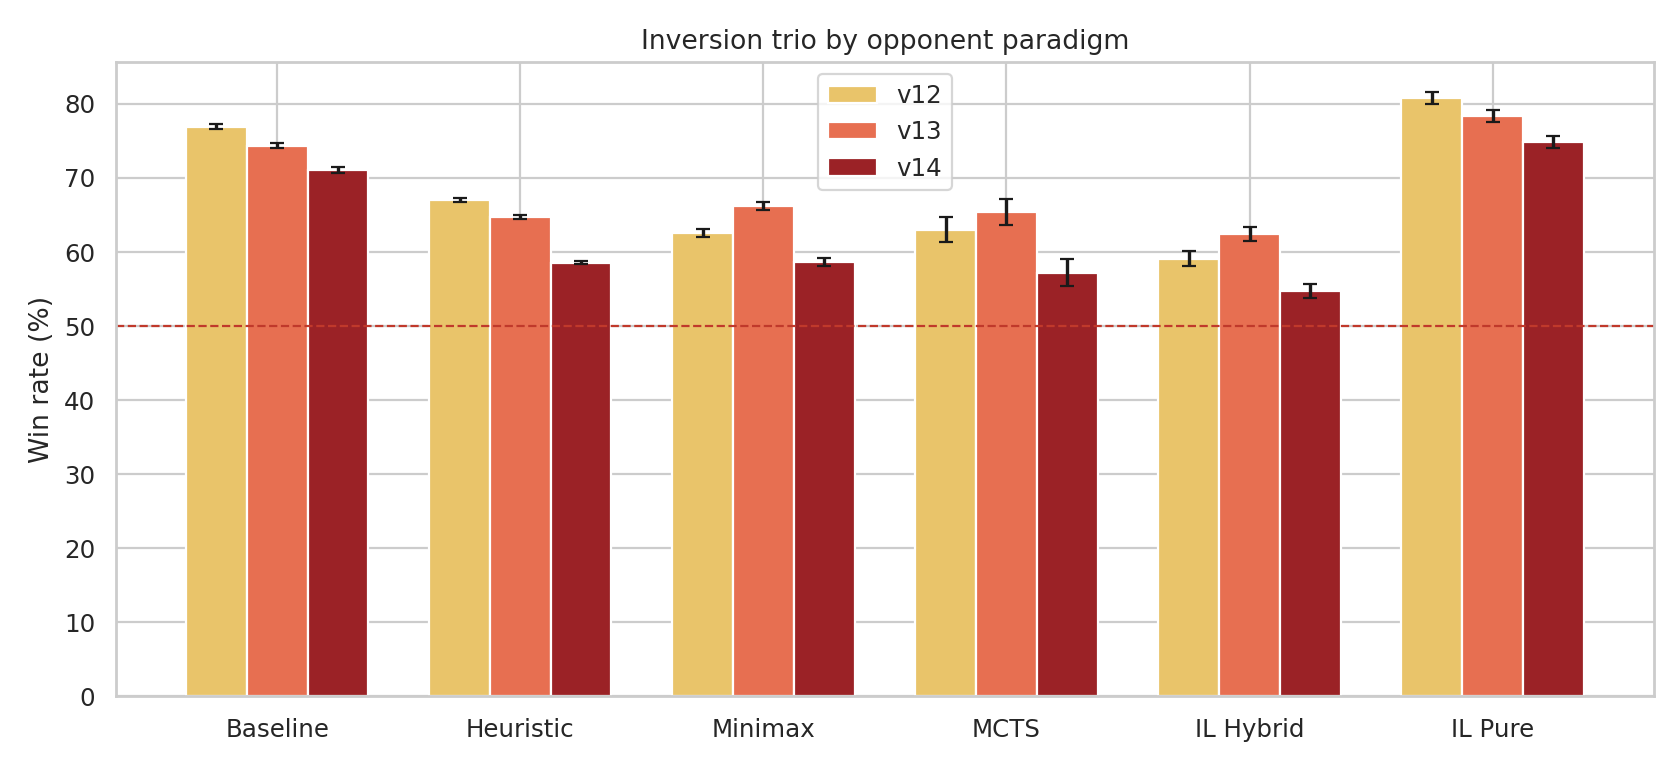
\includegraphics[width=0.95\linewidth]{images/heuristics/heur_wr_by_paradigm.png}
    \caption{Taxa de victòries de la inversió, agregada per paradigma d'oponent. \texttt{v12} és millor contra agents de referència i altres heurístiques; \texttt{v13}, contra minimax, MCTS i imitació híbrida.}
    \label{fig:heur_paradigm}
\end{figure}

En aquest banc de proves, afegir modelatge d'oponents humans redueix el rendiment agent-contra-agent (Figura~\ref{fig:heur_paradigm}). Això indica una possible especialització de domini i justifica mantenir separades la matriu local i l'avaluació pública.

La mostra pública de \texttt{v14} (Secció~\ref{sec:res_ladder}) no permet reordenar \texttt{v12} i \texttt{v14}; de la mateixa manera, la matriu local no permet afirmar quin dels dos obtindria més victòries contra persones.

% ============================================================
\FloatBarrier
\section{Minimax d'un torn}
\label{sec:res_mm}

La pregunta de disseny ---si un maximin d'un torn corregeix \texttt{v14}--- és la de la Secció~\ref{sec:disseny_agents}. Aquí es mesura amb quina freqüència s'executa el mòdul i quan la seva acció difereix de la proposta heurística (Taula~\ref{tab:minimax_head}).

\begin{table}[H]
\centering
\caption{Minimax analític d'un torn (253.000 partides per fila). La cerca s'executa en aproximadament el 16--18\% dels torns. La fulla posicional de \texttt{v16} gairebé no modifica la preparació; el prior de \texttt{v17} redueix la discrepància respecte de \texttt{v14} i obté la taxa més alta de la família.}
\label{tab:minimax_head}
\small
\begin{tabular}{lrrr}
\toprule
 & \textbf{\texttt{v15} HP} & \textbf{\texttt{v16} bonuses} & \textbf{\texttt{v17} prior $+0{,}15$} \\
\midrule
TV global (\%) & 53,80 & 54,30 & \textbf{57,89} \\
IC 95\% (pp) & $\pm 0{,}19$ & $\pm 0{,}19$ & $\pm 0{,}19$ \\
Cerca (\% torns) & 17,6 & 17,6 & 16,3 \\
Discrepància amb \texttt{v14} (\%) & 66,5 & 67,3 & \textbf{36,6} \\
Preparació / partida & 0,21 & 0,21 & 0,21 \\
Perills / partida & 0,05 & 0,04 & 0,04 \\
Tera / partida & 0,40 & 0,39 & 0,38 \\
Pokémon restants & 1,28 & 1,29 & 1,39 \\
\bottomrule
\end{tabular}
\end{table}


\subsection{Freqüència d'intervenció}

Es registren aproximadament 14 comprovacions de debilitament i 4,5 decisions maximin per partida, tal com resumeix l'empremta tàctica de la Figura~\ref{fig:minimax_fp}. La matriu de cerca s'utilitza en el \textbf{16--18\% dels torns}; la resta es resol principalment amb les regles prioritàries heretades.

\begin{quote}
Un agent \texttt{v14} que prioritza debilitaments garantits i aplica una anàlisi maximin d'un torn a les decisions restants.
\end{quote}

Aquest patró és comparable al de \texttt{v21}, que consulta XGBoost en aproximadament el 15\% dels torns, i al de les variants MCTS. Les partides perdudes presenten una discrepància mitjana superior (taxa de \texttt{search\_diff} per torn, detallada a la Figura~\ref{fig:minimax_override}); és una associació, no una prova causal.

\begin{figure}[htbp]
    \centering
    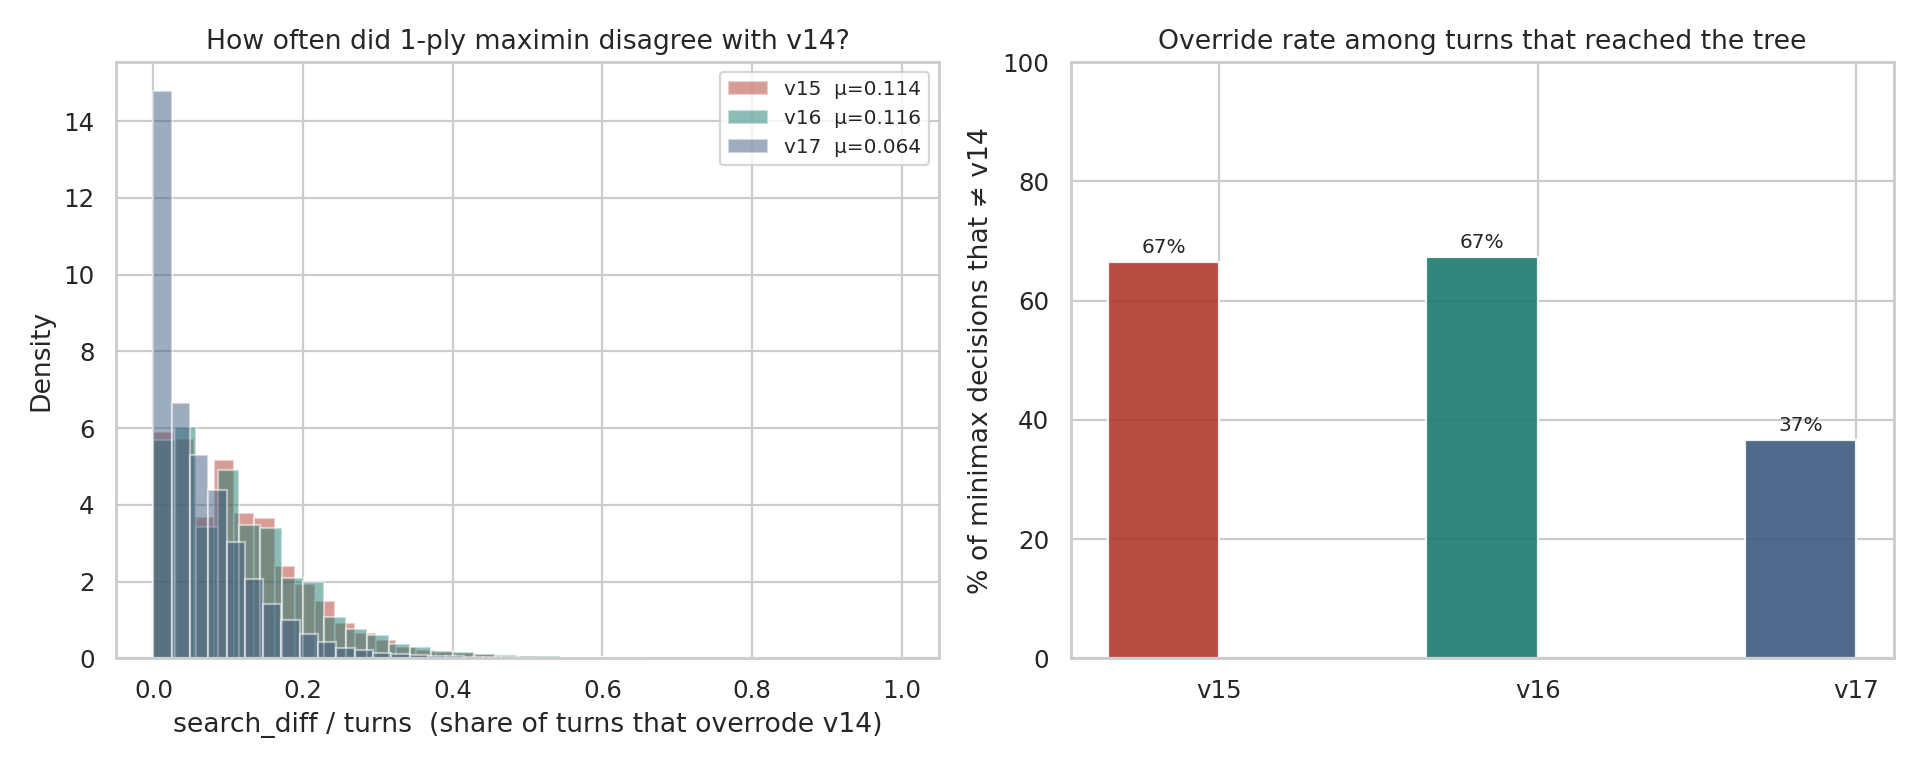
\includegraphics[width=0.92\linewidth]{images/minimax/minimax_override.png}
    \caption{Taxa de discrepància respecte de \texttt{v14} en els torns en què s'executa el maximin. Les barres arrodoneixen a l'enter (67\% / 67\% / 37\%); els valors de la Taula~\ref{tab:minimax_head} són $66{,}5$, $67{,}3$ i $36{,}6$.}
    \label{fig:minimax_override}
\end{figure}

\subsection{\texttt{v16} i l'avaluació de la fulla}

\texttt{v16} incorpora bonificacions per moviments de preparació i perills d'entrada. La taxa global només augmenta 0,50~pp i els enfrontaments directes queden prop del 50\%. Les freqüències de preparació (0,213 i 0,207 per partida) i de perills d'entrada (0,044 i 0,049) pràcticament no canvien. Amb aquesta funció de fulla, el terme de dany rival continua dominant les bonificacions de llarg termini.

La discrepància es manté al voltant del 67\%. Per tant, enriquir la fulla en aquesta magnitud no modifica substancialment la política.

Aquest resultat és coherent amb una limitació d'horitzó: afegir una bonificació estàtica no equival a simular les conseqüències futures d'un moviment de preparació.

\subsection{\texttt{v17}: prior heurístic}

\texttt{v17} afegeix 0,15 al valor de l'acció proposada per \texttt{v14}. La discrepància baixa del $67{,}3\%$ al $36{,}6\%$ i la taxa global augmenta 4,09~pp respecte de \texttt{v15} (diferència altament significativa sobre les 253.000 partides agregades, $z \approx 29{,}3$, $p < 10^{-50}$). En els enfrontaments directes obté $54{,}71\%$ i $54{,}30\%$ contra \texttt{v15} i \texttt{v16} ($n=10.000$; tests de proporció contra paritat $z = 9{,}42$ i $z = 8{,}60$, respectivament, $p < 10^{-17}$ en ambdós casos). El resultat mostra que conservar un prior heurístic és més efectiu, en aquesta implementació, que substituir-lo per la matriu d'un torn.

Contra els comparadors principals, amb $n=10.000$ tret de les cel·les MCTS:

\begin{table}[htbp]
\centering
\small
\caption{Comparativa de les variants Minimax (\texttt{v15}, \texttt{v16}, \texttt{v17}) davant dels principals oponents (taxa de victòries en \%).}
\label{tab:minimax_comparators}
\begin{tabular}{lrrr}
\toprule
Oponent & \texttt{v15} & \texttt{v16} & \texttt{v17} \\
\midrule
\texttt{v12} & 36,04 & 35,92 & \textbf{40,94} \\
\texttt{v13} & 32,82 & 33,50 & 35,10 \\
\texttt{v14} (professor) & 39,43 & 39,56 & \textbf{43,61} \\
Abyssal & 41,72 & 41,86 & \textbf{46,79} \\
\texttt{v20} ($n=1$k) & 39,7 & 44,6 & \textbf{50,4} \\
\texttt{v21} & 43,65 & 44,75 & 47,50 \\
\texttt{v22} & 69,67 & 70,22 & 71,27 \\
\bottomrule
\end{tabular}
\end{table}

\texttt{v17} obté \textbf{43,61\%} contra \texttt{v14}, \textbf{40,94\%} contra \texttt{v12} i 46,79\% contra Abyssal (Taula~\ref{tab:minimax_comparators}). Contra \texttt{v20} obté 50,4\% amb $n=1.000$, un resultat compatible amb rendiments similars en aquell enfrontament.

Cap variant de minimax supera \texttt{v14} o \texttt{v12}. La variant amb millor resultat és precisament la que limita la desviació respecte de l'heurística de partida.

\subsection{Canvis, durada i supervivència}

Pel que fa a la durada dels combats i l'estat final de l'equip, les tres variants de minimax presenten una durada pràcticament coincident, situada al voltant dels 19 torns de mitjana. La millora de \texttt{v17} no prové, per tant, d'allargar sistemàticament les batalles: el seu avantatge rau en una major conservació de recursos, ja que conserva de mitjana 1,39 membres de l'equip al final de la partida, enfront dels 1,28--1,29 membres de \texttt{v15} i \texttt{v16}. Aquesta diferència augmenta significativament la proporció de partides guanyades amb dos o tres membres restants, un patró coherent amb una reducció de decisions maximin agressives que exposaven innecessàriament el Pokémon actiu.

D'altra banda, en la distribució de canvis, \texttt{v17} presenta una mediana superior de canvis voluntaris i de canvis decidits pel mòdul de cerca respecte de \texttt{v15} i \texttt{v16}, tot i discrepar menys de la política base de \texttt{v14}. Aquesta combinació de «més canvis decidits per cerca» i «menys discrepància» no és contradictòria: indica que, quan \texttt{v14} ja aconsella canviar de Pokémon, el prior de $+0{,}15$ afegit a \texttt{v17} reforça el maximin per consolidar aquesta mateixa decisió en lloc de forçar un atac de baix valor. El guany no prové d'un increment indiscriminat del volum brut de canvis, sinó de preservar el criteri de canvi heurístic en estats on una matriu de cerca d'un sol torn manca de la profunditat temporal necessària per ponderar l'atrició a llarg termini, un efecte que es tradueix en un increment de victòries davant d'heurístiques i MCTS (Figura~\ref{fig:minimax_paradigm}).

\begin{figure}[htbp]
    \centering
    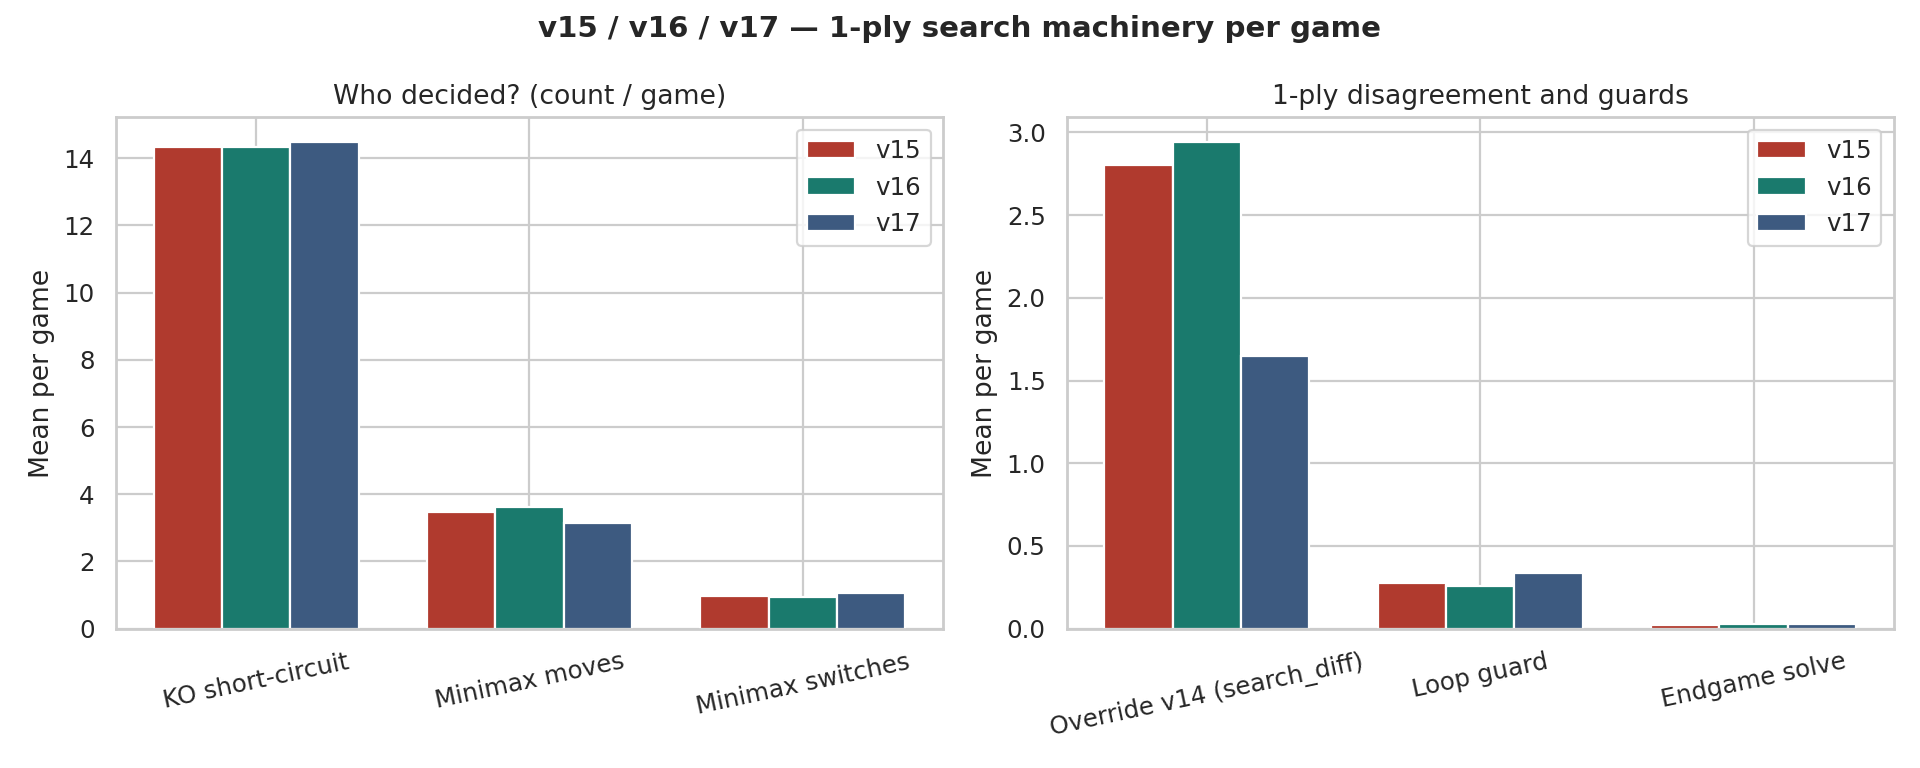
\includegraphics[width=0.92\linewidth]{images/minimax/minimax_fingerprint_bars.png}
    \caption{Empremta \texttt{v15}--\texttt{v17}: KO checks $\sim$14, cerca $\sim$16--18\% dels torns, Tera $\sim$0,39 (nivell \texttt{v14}, no \texttt{v12}).}
    \label{fig:minimax_fp}
\end{figure}

\begin{figure}[htbp]
    \centering
    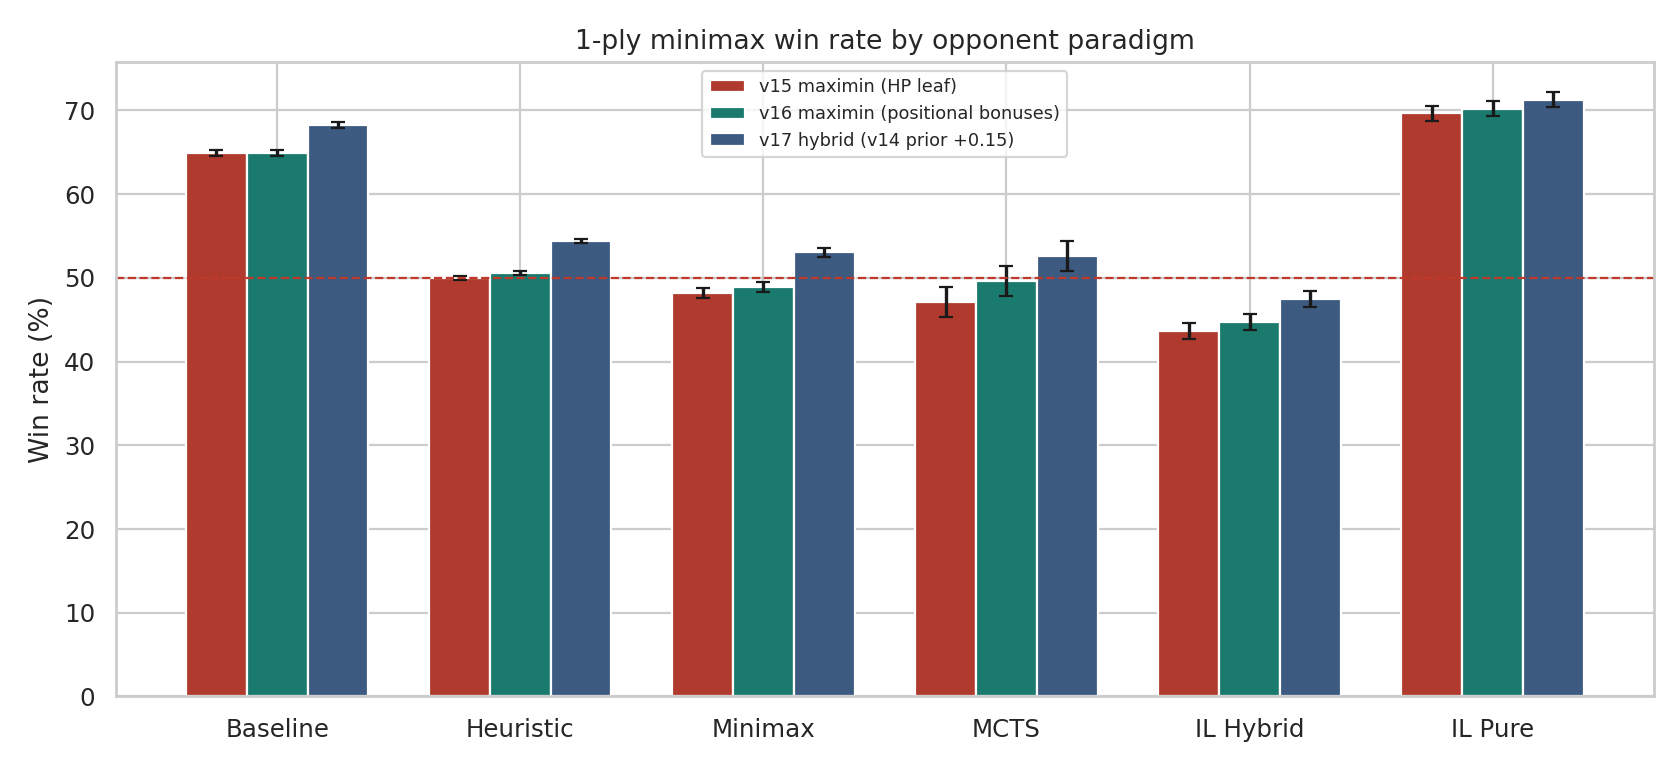
\includegraphics[width=0.92\linewidth]{images/minimax/minimax_wr_by_paradigm.png}
    \caption{Taxa de victòries del minimax per família d'oponent. El prior de \texttt{v17} s'associa amb les millores principals contra heurístiques i MCTS.}
    \label{fig:minimax_paradigm}
\end{figure}

% ============================================================
\FloatBarrier
\section{MCTS ras: UCB a l'arrel i simulacions de cinc torns}
\label{sec:res_mcts}

\textbf{Totes les cel·les d'aquesta secció tenen $n=1.000$} ($\pm 3$~pp, Taula~\ref{tab:ci_n}). La mitjana global de les files MCTS també té una ponderació diferent de la de les files no MCTS. La pregunta de disseny ---si cinc torns simulats superen l'horitzó de \texttt{v14}--- és la de la Secció~\ref{sec:disseny_agents}, amb els registres principals resumits a la Taula~\ref{tab:mcts_head}.

\begin{table}[H]
\centering
\caption{IS-MCTS (100 simulacions $\times$ 5 torns de \texttt{LocalSim}). \textbf{Totes les cel·les $n=1.000$}; 28.000 partides per agent; IC global $\approx\pm 0{,}58$~pp, IC per cel·la $\approx\pm 3{,}1$~pp. Una fulla més rica (\texttt{v19}) no ajuda. PUCT amb prior 0,70 sobre \texttt{v14} (\texttt{v20}) és l'única millora, perquè discrepa \emph{menys}.}
\label{tab:mcts_head}
\small
\begin{tabular}{lrrr}
\toprule
 & \textbf{\texttt{v18} UCB1 HP} & \textbf{\texttt{v19} UCB1 pos.} & \textbf{\texttt{v20} PUCT 0,70} \\
\midrule
WR global (\%) & 54,02 & 53,29 & \textbf{59,66} \\
Cerca (\% torns) & 18,1 & 17,6 & 15,5 \\
Override de \texttt{v14} (\%) & 71,3 & 71,1 & \textbf{18,7} \\
Setup / partida & 0,22 & 0,22 & 0,20 \\
Hazards / partida & 0,05 & 0,05 & 0,04 \\
Tera / partida & 0,41 & 0,39 & 0,39 \\
Mons restants (nosaltres) & 1,21 & 1,22 & 1,40 \\
\bottomrule
\end{tabular}
\end{table}


\texttt{v20} obté una taxa superior a \texttt{v18} en els \textbf{28 enfrontaments} (diferència mitjana de 5,64~pp). \texttt{v18} i \texttt{v19} queden prop del 50\% en l'enfrontament directe, mentre que \texttt{v20} obté aproximadament 56,6\% contra tots dos. En aquest pressupost, enriquir només la funció de fulla de \texttt{v19} no aporta una millora observable.

\subsection{Freqüència d'intervenció}

Es registren aproximadament 14 comprovacions de debilitament i 3--4 decisions MCTS per partida. La cerca intervé en el \textbf{15--18\%} dels torns:

\begin{quote}
Un agent basat en \texttt{v14} que prioritza els debilitaments garantits i aplica 100 simulacions de cinc torns a les decisions restants.
\end{quote}

Quan s'activa una drecera prèvia, les 100 simulacions no s'executen. Per tant, la cerca només pot modificar el subconjunt de decisions que arriba a l'arrel.

\begin{figure}[htbp]
    \centering
    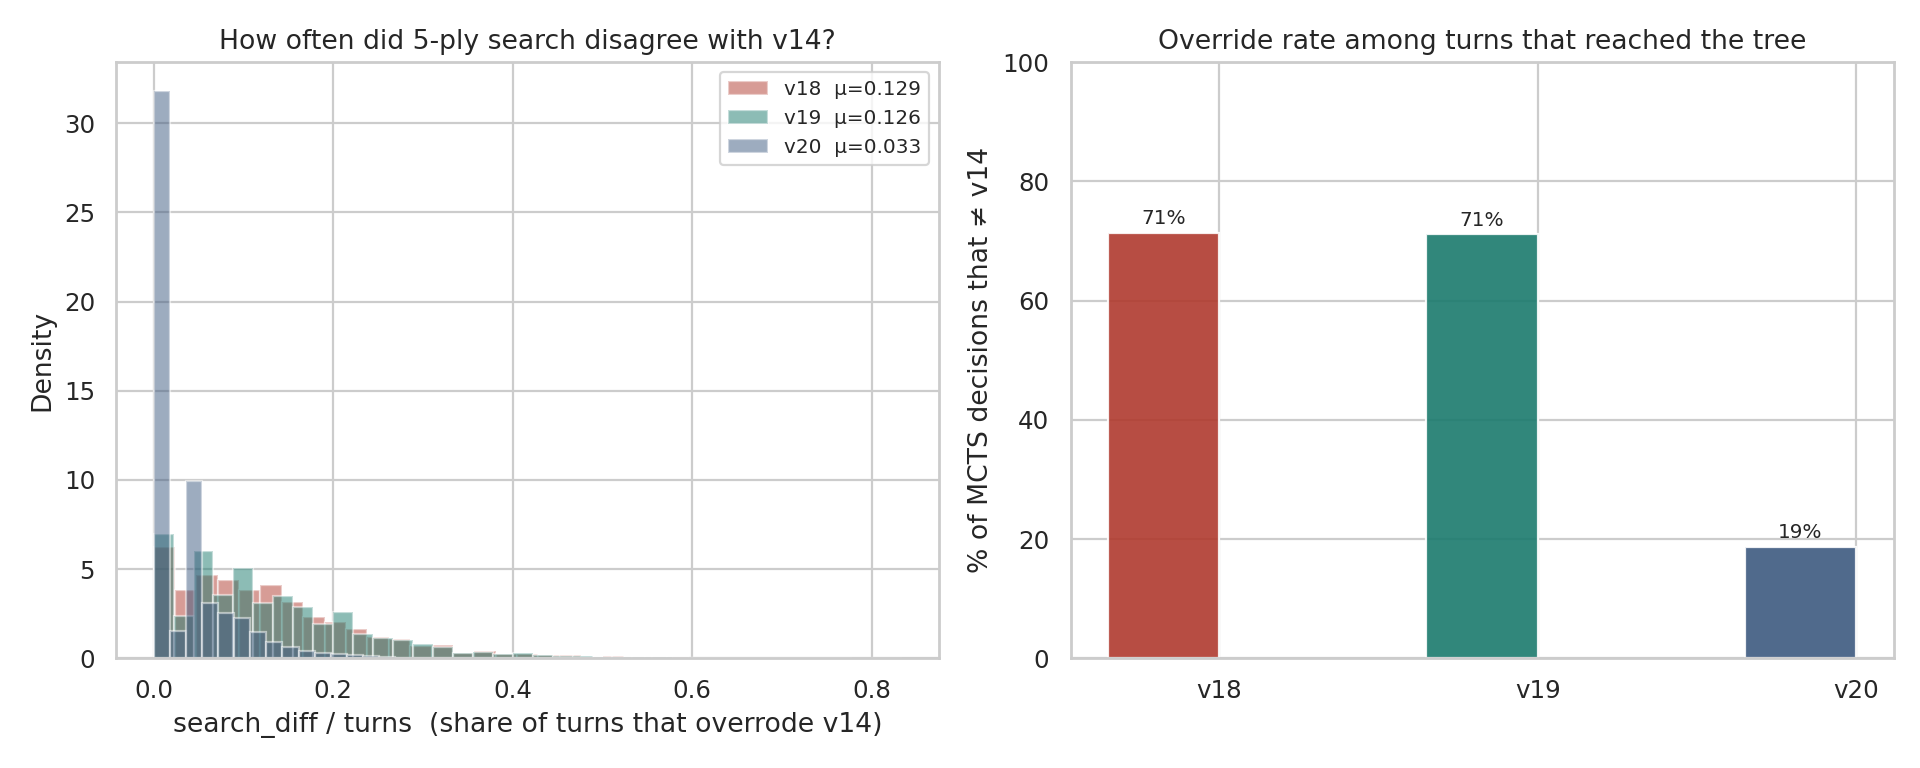
\includegraphics[width=0.92\linewidth]{images/mcts/mcts_override.png}
    \caption{Taxa de discrepància respecte de \texttt{v14} entre les decisions de cerca. Les barres arrodoneixen a l'enter (71\% / 71\% / 19\%); els valors de la Taula~\ref{tab:mcts_head} són $71{,}3$, $71{,}1$ i $18{,}7$.}
    \label{fig:mcts_override}
\end{figure}

\subsection{Discrepància i resultat}

\texttt{search\_diff} indica que la simulació ha canviat l'acció proposada per \texttt{v14}. Entre els torns en què s'executa:

\begin{itemize}
    \item \texttt{v18}/\texttt{v19} discrepen de \texttt{v14} en el \textbf{71,3\%} i el \textbf{71,1\%} de les decisions de cerca, respectivament, mentre que el prior PUCT de \texttt{v20} redueix aquesta taxa al 18,7\% (Figura~\ref{fig:mcts_override}).
    \item Les partides perdudes presenten una discrepància superior. Aquest patró pot reflectir decisions pitjors, estats més difícils o ambdues coses.
    \item Les simulacions de cinc torns i la funció de fulla basada en HP poden afavorir el dany immediat davant d'efectes diferits.
\end{itemize}

\texttt{v19} incorpora una fulla posicional, però manté una discrepància del 71,1\% i una taxa global 0,7~pp inferior a \texttt{v18}. Les dades no mostren que aquest canvi de fulla resolgui les limitacions del pressupost, de la política de simulació o de la informació oculta.

\subsection{PUCT i el prior heurístic}

Amb un prior de 0,70 sobre \texttt{v14}, la discrepància baixa al \textbf{18,7\%}. \texttt{v20} obté una taxa global descriptiva de \textbf{59,66\%} i conserva 1,40 Pokémon de mitjana al final.

Les diferències de \texttt{v20} respecte de \texttt{v18} són especialment grans contra \texttt{v17} (+11,1~pp), \texttt{v13} (+10,5), \texttt{v15} (+9,8) i \texttt{v12} (+8,7). Contra \texttt{random}, la diferència és de 0,3~pp i queda molt per sota de la precisió de la cel·la.

Amb aquest pressupost, la millor variant MCTS és la que utilitza les simulacions per ajustar un prior heurístic, no la que substitueix l'heurística amb UCB1 sense guia.

\subsection{Indicadors d'efectes diferits}

A la Taula~\ref{tab:deferred_effects} es resumeixen les taxes d'activació de mecàniques diferides per partida segons paradigma.

\begin{table}[htbp]
\centering
\small
\caption{Freqüències mitjanes d'activació de mecàniques diferides (\emph{setup}, \emph{hazards} i Teracristal·lització per partida) segons paradigma.}
\label{tab:deferred_effects}
\begin{tabular}{lrrr}
\toprule
 & Setup/partida & Hazards/partida & Tera/partida \\
\midrule
\texttt{v12} (comparador) & $\sim$1,75 & $\sim$0,18 & $\sim$0,96 \\
\texttt{v14} (professor) & $\sim$0,21 & $\sim$0,03 & $\sim$0,34 \\
Minimax d'un torn \texttt{v15}--\texttt{v17} & 0,21 & 0,04--0,05 & 0,38--0,40 \\
MCTS de cinc torns \texttt{v18}--\texttt{v20} & 0,20--0,22 & 0,04--0,05 & 0,39--0,41 \\
\bottomrule
\end{tabular}
\end{table}

Les freqüències de preparació i perills d'entrada es mantenen a nivells semblants als de \texttt{v14}, no als de \texttt{v12}. Les simulacions de cinc torns no recuperen, amb aquesta política, el comportament diferit observat a l'heurística amb millor taxa.

\texttt{v20} presenta més \texttt{search\_switches} (aproximadament 36\% de les decisions de cerca, davant del 16\% a \texttt{v18}) i menys discrepància total. Això indica que PUCT reforça sovint els canvis ja proposats per \texttt{v14}.

\subsection{Comparació amb els agents de referència}

\begin{table}[htbp]
\centering
\small
\caption{Rendiment de les variants MCTS (\texttt{v18}, \texttt{v19}, \texttt{v20}) davant dels oponents de referència (taxa de victòries en \%).}
\label{tab:mcts_comparators}
\begin{tabular}{lrrr}
\toprule
Oponent & \texttt{v18} & \texttt{v19} & \texttt{v20} \\
\midrule
\texttt{v12} & 34,0 & 33,1 & \textbf{42,7} \\
\texttt{v13} & 28,6 & 34,1 & 39,1 \\
\texttt{v14} & 40,0 & 41,7 & \textbf{47,0} \\
Abyssal & 42,2 & 38,7 & \textbf{49,0} \\
\texttt{v15} & 49,3 & 51,6 & \textbf{59,1} \\
\texttt{v17} & 44,7 & 45,3 & 55,8 \\
\texttt{v21} & 44,1 & 46,5 & 49,6 \\
\texttt{v22} & 71,1 & 66,9 & 73,0 \\
\bottomrule
\end{tabular}
\end{table}

\texttt{v20} obté \textbf{47,0\%} contra \texttt{v14}, \textbf{42,7\%} contra \texttt{v12} i \textbf{49,0\%} contra Abyssal (Taula~\ref{tab:mcts_comparators}). Amb $n=1.000$, el primer i el tercer resultat són compatibles amb la paritat del 50\% ($z = -1{,}90$, $p = 0{,}057$ i $z = -0{,}63$, $p = 0{,}53$, no significatius al nivell $\alpha=0{,}05$). En canvi, el desavantatge davant \texttt{v12} és significatiu ($z = -4{,}62$, $p < 10^{-5}$), i els avantatges davant \texttt{v15} (59,1\%, $z = 5{,}76$, $p < 10^{-8}$) i \texttt{v22} (73,0\%, $z = 14{,}55$, $p < 10^{-15}$) són estadísticament inequívocs.

Per blocs (Figura~\ref{fig:mcts_paradigm}), \texttt{v20} obté 69,9\% contra agents de referència, 56,7\% contra heurístiques i 57,4\% contra minimax. \texttt{v18}/\texttt{v19} se situen prop del 50\% contra heurístiques i per sota del 50\% contra minimax.

L'MCTS ras amb 100 simulacions de cinc torns no supera \texttt{v12} ni aporta evidència de superar \texttt{v14}. Dins de la família, el prior heurístic de \texttt{v20} és el canvi associat amb la millora principal.

\subsection{Canvis, durada i supervivència}

En l'anàlisi de la durada dels combats i la supervivència de l'equip, \texttt{v20} conclou les batalles lleugerament abans (18,33 torns de mitjana) i conserva 1,40 membres de l'equip al final de la partida, davant dels 1,21--1,22 membres que aconsegueixen preservar les variants d'UCB1 pur (\texttt{v18} i \texttt{v19}). El patró de \texttt{v20} no és, per tant, el d'una política excessivament defensiva que es limita a prolongar els enfrontaments: tanca les partides amb més rapidesa i preservant més recursos. Una explicació plausible és que el guiatge heurístic del prior desaconsella branques de simulació miops que opten per dany immediat a costa d'un enfrontament clarament desfavorable al torn següent.

Pel que fa a la dinàmica de canvis, l'algorisme PUCT augmenta de manera substancial la fracció de decisions de cerca que acaben en canvi i n'eixampla la distribució de canvis voluntaris. Mentre que \texttt{v18} gairebé mai escull un canvi des de l'arrel en la mediana de partides, a \texttt{v20} aproximadament un terç de les decisions preses pel mòdul de cerca corresponen a canvis de Pokémon. Com que al mateix temps la taxa de discrepància \texttt{search\_diff} cau fins al 18,7\%, aquests canvis solen coincidir amb la recomanació del coneixement expert de \texttt{v14}. Aquesta convergència reforça la interpretació que la millora de PUCT rau en consolidar i no degradar la posició tàctica proposada per l'heurística (com reflecteix l'empremta tàctica de la Figura~\ref{fig:mcts_fp}), més que en la descoberta d'estratègies noves en un horitzó de cinc torns.

\begin{figure}[htbp]
    \centering
    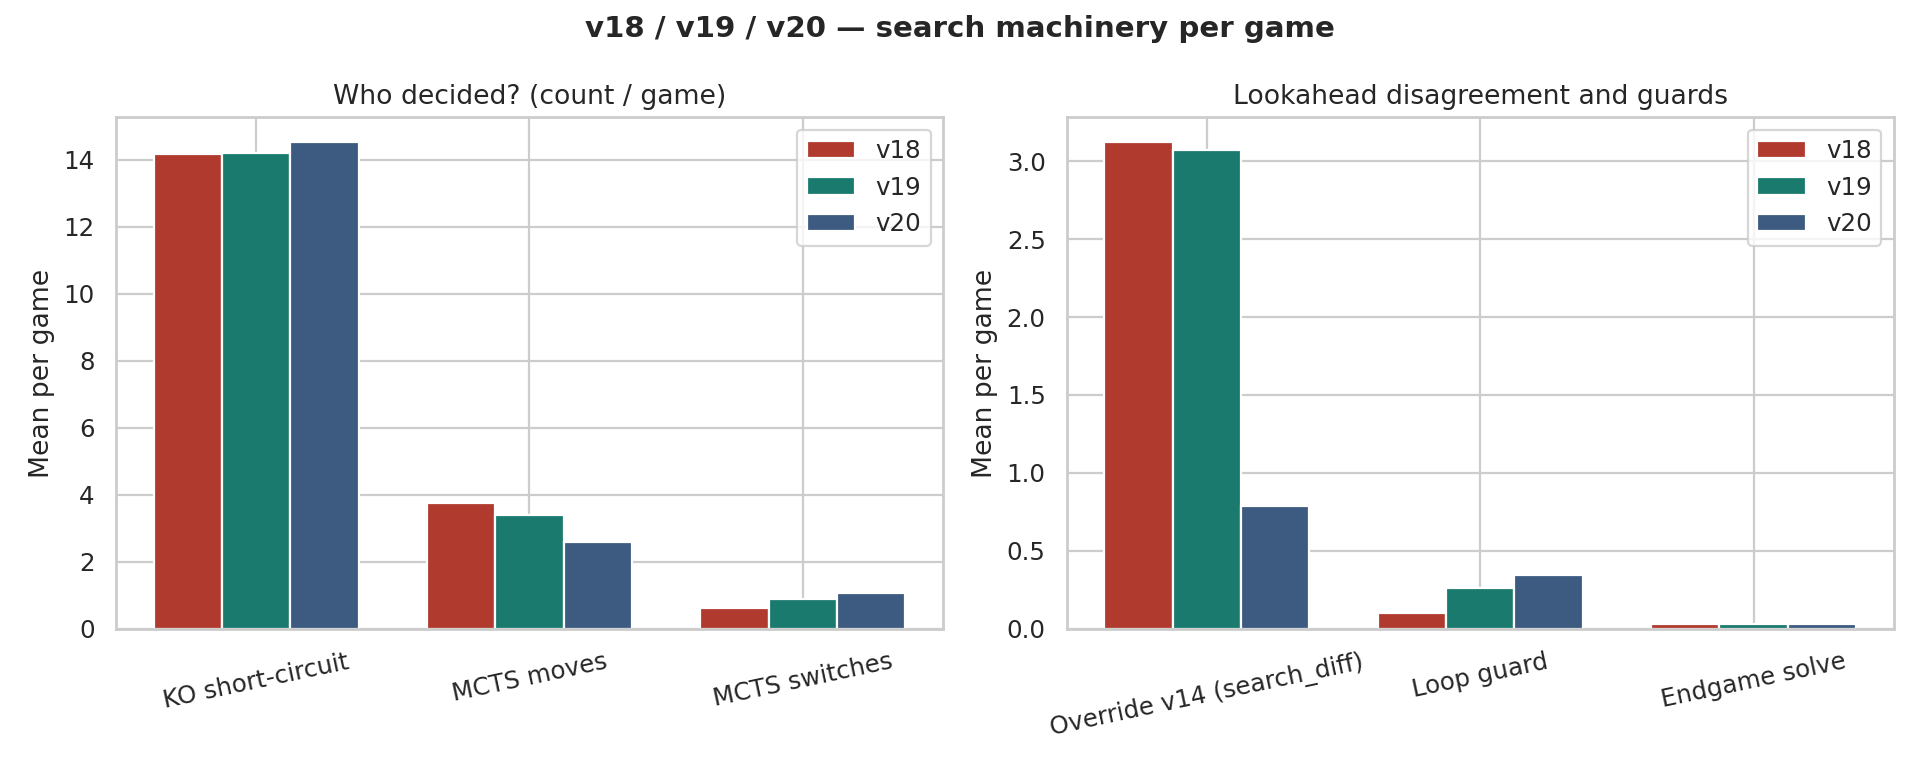
\includegraphics[width=0.92\linewidth]{images/mcts/mcts_fingerprint_bars.png}
    \caption{Empremta MCTS. Cerca 15--18\% dels torns (\texttt{v20}: $15{,}5\%$); KO $\sim$14/partida. \texttt{v20} busca menys i acaba amb més HP. $n=1.000$ per oponent.}
    \label{fig:mcts_fp}
\end{figure}

\begin{figure}[htbp]
    \centering
    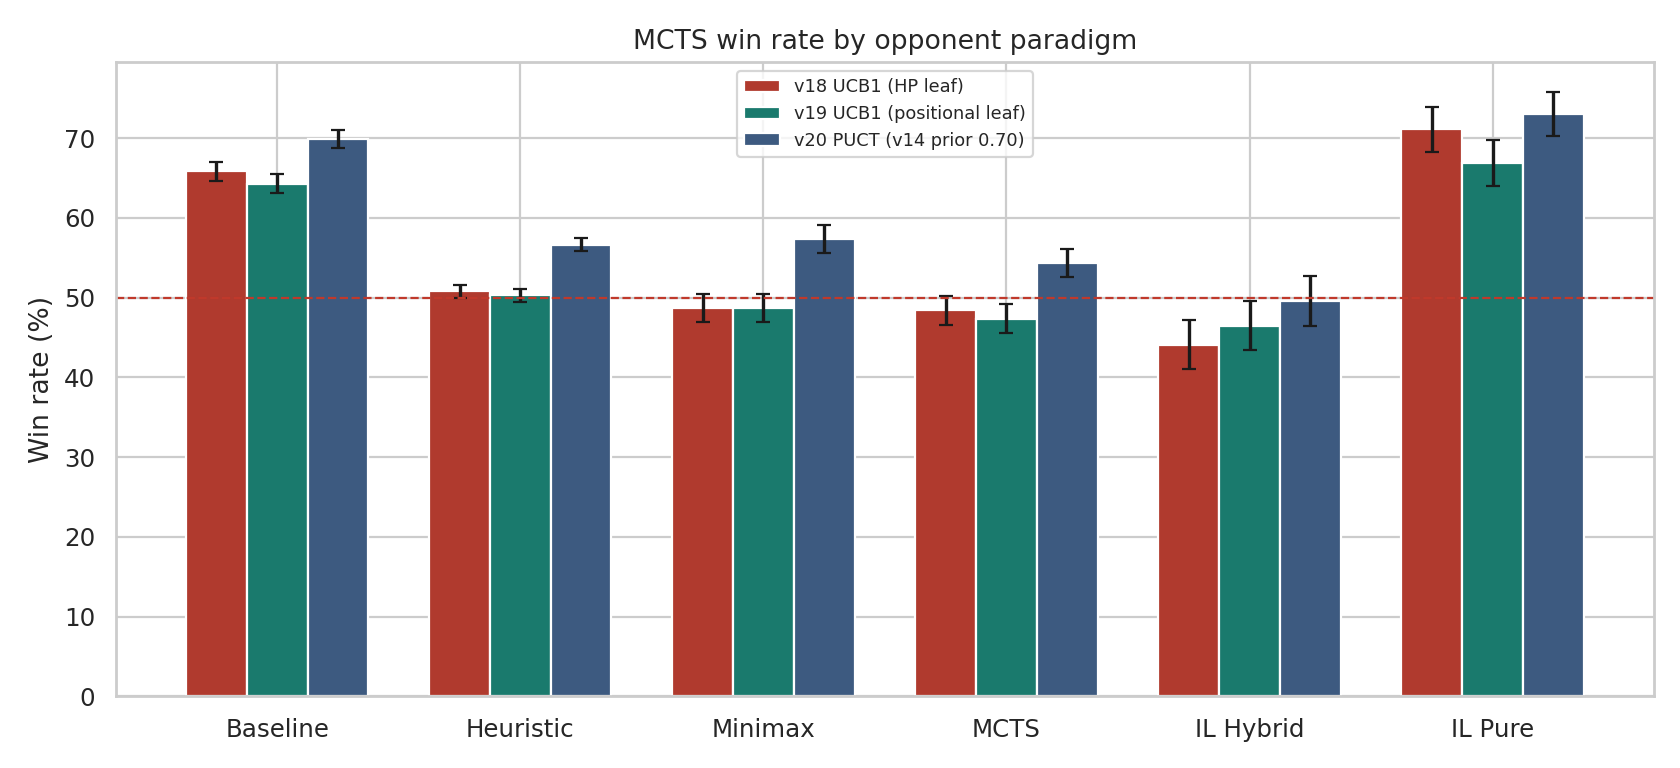
\includegraphics[width=0.92\linewidth]{images/mcts/mcts_wr_by_paradigm.png}
    \caption{Taxa de victòries d'MCTS per paradigma d'oponent ($n=1.000$ a cada cel·la). PUCT millora principalment contra heurístiques i minimax.}
    \label{fig:mcts_paradigm}
\end{figure}

% ============================================================
\FloatBarrier
\section{Aprenentatge per imitació: dues formes d'execució}
\label{sec:res_il}

Les dues variants comparteixen el classificador XGBoost i el llindar $\tau=0{,}5525$ del Capítol~\ref{chap:implementacio}, però difereixen en la selecció de l'acció concreta (Taula~\ref{tab:il_head}).

\begin{table}[H]
\centering
\caption{Imitació amb el mateix classificador XGBoost ($\tau=0{,}5525$) i dues formes d'execució (253.000 partides per fila). \texttt{v21} consulta el model en el 15\% dels torns; \texttt{v22}, en el 80\%, sense proteccions de debilitament, i activa la protecció de bucle en el 97\% de les partides.}
\label{tab:il_head}
\small
\begin{tabular}{lrr}
\toprule
 & \textbf{\texttt{v21} híbrid} & \textbf{\texttt{v22} atributs} \\
\midrule
TV global (\%) & \textbf{58,71} $\pm 0{,}19$ & 33,49 $\pm 0{,}18$ \\
Torns mitjans & 18,20 & 20,07 \\
Pokémon restants & 1,33 & 0,70 \\
Canvis voluntaris / partida & 1,98 & 3,72 \\
XGBoost (\% torns) & 15,2 & 79,9 \\
Entre decisions XGB, \% canvis & 35,5 & 15,2 \\
Mitjana $p(\mathrm{canvi})$ & 0,080 & 0,351 \\
Proteccions de KO / partida & 13,85 & \textbf{0} \\
Resolucions de final / partida & 0,032 & \textbf{0} \\
Proteccions de bucle / partida (\% partides) & 0,38 (33\%) & 1,92 (\textbf{97\%}) \\
\bottomrule
\end{tabular}
\end{table}


\texttt{v21} obté una taxa superior a \texttt{v22} en els \textbf{28 enfrontaments} (Figura~\ref{fig:il_scatter}), amb una diferència mitjana de 25,2~pp. En el cara a cara, les dues orientacions són 71,74\% i 29,07\%; l'autojoc queda prop del 50\%. A \texttt{v22}, els comptadors \texttt{ko\_guards}, \texttt{endgame\_solves}, \texttt{ko\_checks} i \texttt{search\_*} són zero, fet que confirma que no executa les dreceres de \texttt{v14}, com s'observa a l'empremta tàctica comparativa de la Figura~\ref{fig:il_fp}.

\begin{figure}[htbp]
    \centering
    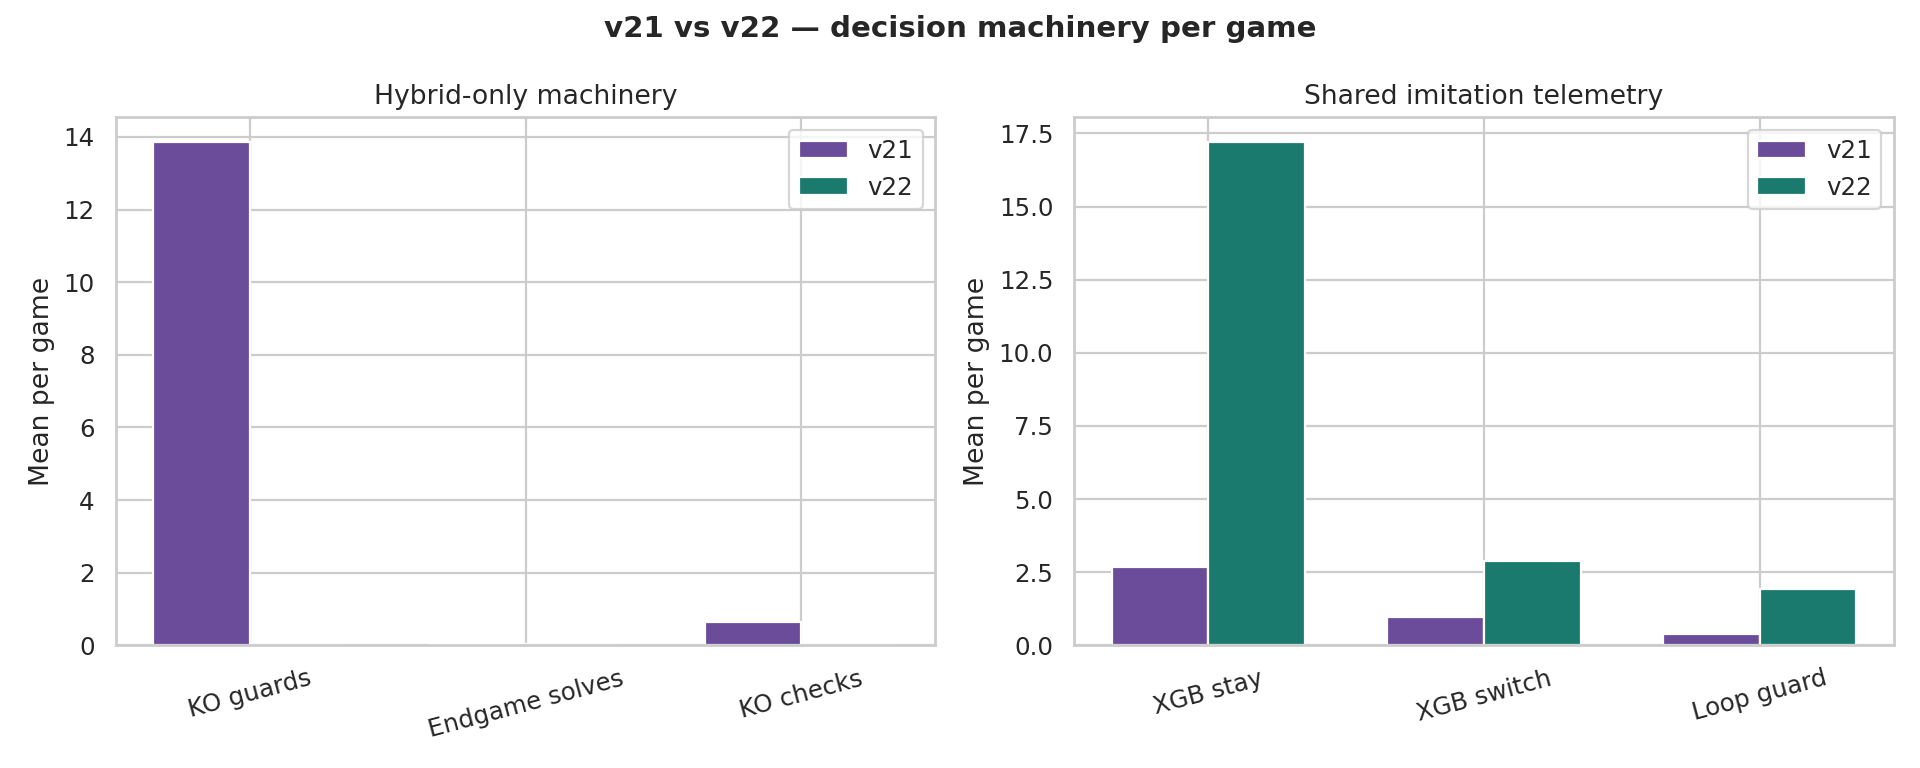
\includegraphics[width=0.92\linewidth]{images/il/il_fingerprint_bars.png}
    \caption{Empremta dels agents d'imitació. \texttt{v21} registra aproximadament 14 proteccions de debilitament per partida; \texttt{v22} no. El panell dret mostra que \texttt{v22} consulta XGBoost moltes més vegades i activa més sovint la protecció de bucle.}
    \label{fig:il_fp}
\end{figure}

\subsection{Rendiment dins de la matriu}

\texttt{v21} obté una taxa global descriptiva de 58,71\%, propera a \texttt{v9}/\texttt{v11}. \texttt{v22} obté 33,49\%, per sota de \texttt{v1} (44,25\%). En l'enfrontament directe, \texttt{v1} guanya el 65,72\% de les partides contra \texttt{v22}.

Enfrontaments de referència ($n=10.000$, tret de \texttt{v20}, Taula~\ref{tab:il_comparators}):

\begin{table}[htbp]
\centering
\small
\caption{Comparació de rendiment dels models d'imitació jeràrquica (\texttt{v21}, \texttt{v22}) enfront de la cerca i referències (taxa de victòries en \%).}
\label{tab:il_comparators}
\begin{tabular}{lrrrrr}
\toprule
 & contra \texttt{v12} & contra \texttt{v13} & contra \texttt{v14} & contra Abyssal & contra SimpleH \\
\midrule
\texttt{v21} & 41,28 & 38,39 & 45,43 & 46,98 & 47,76 \\
\texttt{v17} & 40,94 & 35,10 & 43,61 & 46,79 & 46,75 \\
\texttt{v20} ($n=1$k) & 42,7 & 39,1 & 47,0 & 49,0 & 49,2 \\
\texttt{v22} & 19,80 & 22,03 & 25,81 & 22,90 & 21,73 \\
\bottomrule
\end{tabular}
\end{table}

\texttt{v14} obté 54,74\% contra \texttt{v21}, i l'orientació recíproca és 45,43\%. Per tant, afegir el model de decisió atacar/canviar no millora \texttt{v14} en aquest enfrontament. Les taxes contra Abyssal són 46,98\% i 51,36\%, respectivament.

\subsection{Pes efectiu del model a \texttt{v21}}

Només el \textbf{15\%} dels torns arriben a XGBoost (Figura~\ref{fig:il_fire}); les regles prèvies de \texttt{v14} resolen la resta. En els torns consultats, la probabilitat mitjana de canvi és 0,08, molt inferior a $\tau=0{,}5525$. En conseqüència, el model sol indicar que l'agent es mantingui al camp i \texttt{v14} selecciona el moviment.

Descripció honesta:

\begin{quote}
Un agent \texttt{v14} que, en una fracció minoritària dels torns, consulta un model d'imitació per decidir si convé canviar i delega l'execució concreta a la mateixa heurística.
\end{quote}

La capa d'imitació funciona, doncs, com un \textbf{prior sobre el moment de canviar}, no com un motor tàctic complet. Aquesta descripció és important per no atribuir tot el rendiment de \texttt{v21} al model supervisat.

La comparació mostra que la decisió d'alt nivell es pot integrar de manera útil quan l'acció concreta queda restringida per una política competent. No mostra que el classificador, per si sol, reprodueixi el joc expert.

\begin{figure}[htbp]
    \centering
    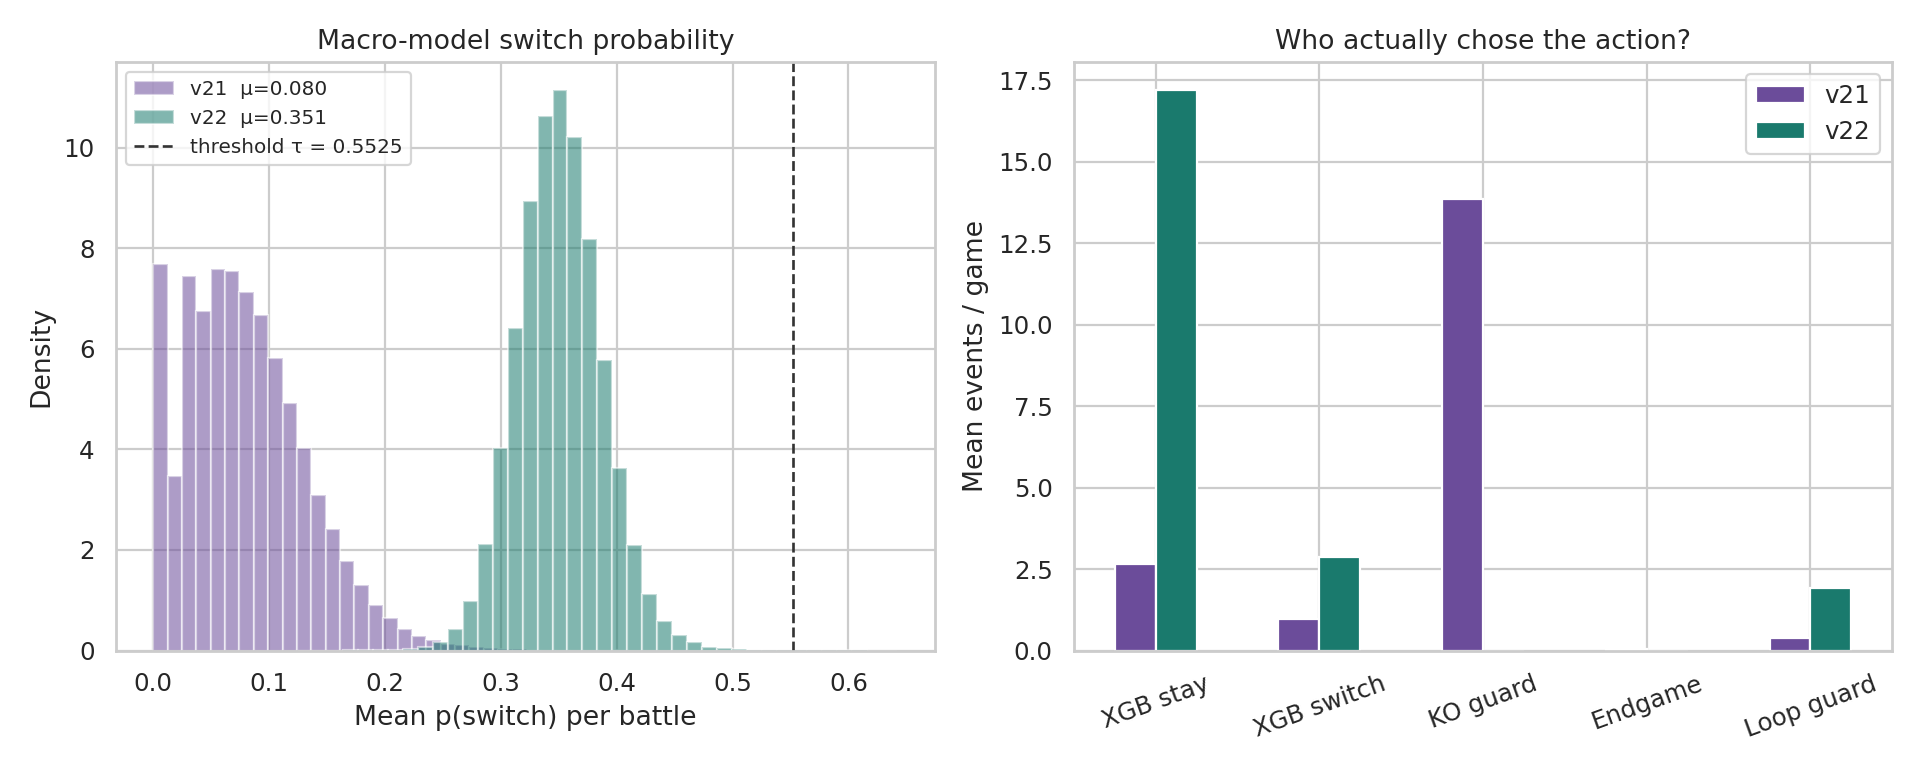
\includegraphics[width=0.92\linewidth]{images/il/il_policy_firing.png}
    \caption{Freqüència d'ús de la política apresa. XGBoost intervé en el 15\% dels torns de \texttt{v21} i en el 80\% dels de \texttt{v22}.}
    \label{fig:il_fire}
\end{figure}

\subsection{Factors que limiten \texttt{v22}}

\begin{enumerate}
    \item \textbf{Semàntica de l'acció.} El primer model només prediu $\{\mathrm{atacar},\mathrm{canviar}\}$ i el segon puntua atributs de candidats sintetitzats. Es perd informació sobre la identitat i el context del moviment.
    \item \textbf{Biaix d'exposició.} Una decisió deficient pot portar la política a estats poc representats a les repeticions. La protecció de bucle s'activa en el \textbf{97\%} de les partides de \texttt{v22}, que també són més llargues i acaben amb menys Pokémon disponibles.
    \item \textbf{Absència de restriccions tàctiques.} \texttt{v21} preserva els debilitaments garantits abans de consultar el model; \texttt{v22} no. La freqüència de Teracristal·lització de \texttt{v22} és alta (gairebé una vegada per partida, enfront d'un ús selectiu i conservador a \texttt{v21} heretat de \texttt{v14}, $\sim 0{,}34$ per partida), però la freqüència per si sola no informa de la qualitat del moment triat.
\end{enumerate}

En aquesta implementació, el resultat depèn tant de \emph{què} s'imita ---la decisió atacar/canviar--- com de \emph{qui} executa l'acció concreta. Disposar d'1,12 milions de torns no compensa una representació que no modela directament la selecció completa de moviments i canvis.

El contrast entre \texttt{v21} i \texttt{v22} no compara únicament dos models d'imitació: també compara una arquitectura jeràrquica amb una execució basada en atributs. Aquesta confusió de factors impedeix atribuir els 25,2~pp exclusivament a una sola decisió de disseny, però demostra la importància de l'executor.

\subsection{Canvis, durada i supervivència}

Pel que fa a la durada de les partides i l'estat final de l'equip, \texttt{v22} registra partides significativament més llargues (amb una mitjana de 20,07 torns) però conclou amb només 0,70 membres de l'equip disponibles de mitjana, en clar contrast amb els 1,33 membres que aconsegueix preservar \texttt{v21}. Aquesta major durada temporal de \texttt{v22} no és en cap cas indicativa de control tàctic o domini posicional: en anar acompanyada d'un nombre tan reduït de supervivents i d'una taxa global de victòria molt menor (33,49\%), reflecteix una dinàmica de canvis que retarda el debilitament inevitable sense arribar a estabilitzar mai la posició. Aquest patró concorda plenament amb el biaix d'exposició de l'aprenentatge per imitació: després d'un canvi subòptim o descontextualitzat, el model es veu obligat a prendre decisions successives en estats allunyats de la distribució de les trajectòries humanes d'entrenament, repercutint en una pèrdua d'eficàcia transversal en tots els paradigmes rivals (Figura~\ref{fig:il_paradigm}).

Aquesta dinàmica es reflecteix directament en la distribució dels canvis. Mentre que els canvis forçats presenten volums similars entre totes dues variants (en dependre primordialment dels debilitaments soferts), la diferència fonamental rau en els canvis voluntaris i en les consultes a XGBoost: \texttt{v22} executa aproximadament el doble de canvis voluntaris que \texttt{v21} i rep moltes més instruccions de canvi del classificador. La distribució de \texttt{v22} es concentra al voltant de 3 o 4 canvis voluntaris per partida, mentre que \texttt{v21} en realitza habitualment entre 1 i 2. Si es combina aquest patró amb el fet que el mecanisme de protecció contra bucles de canvis s'activa en el 97\% de les partides de \texttt{v22}, l'evidència suggereix que el factor limitant no és la manca de propensió al canvi, sinó l'absència d'un executor capaç de ponderar el destí de la transició i el cost tàctic de revertir-la.

\begin{figure}[htbp]
    \centering
    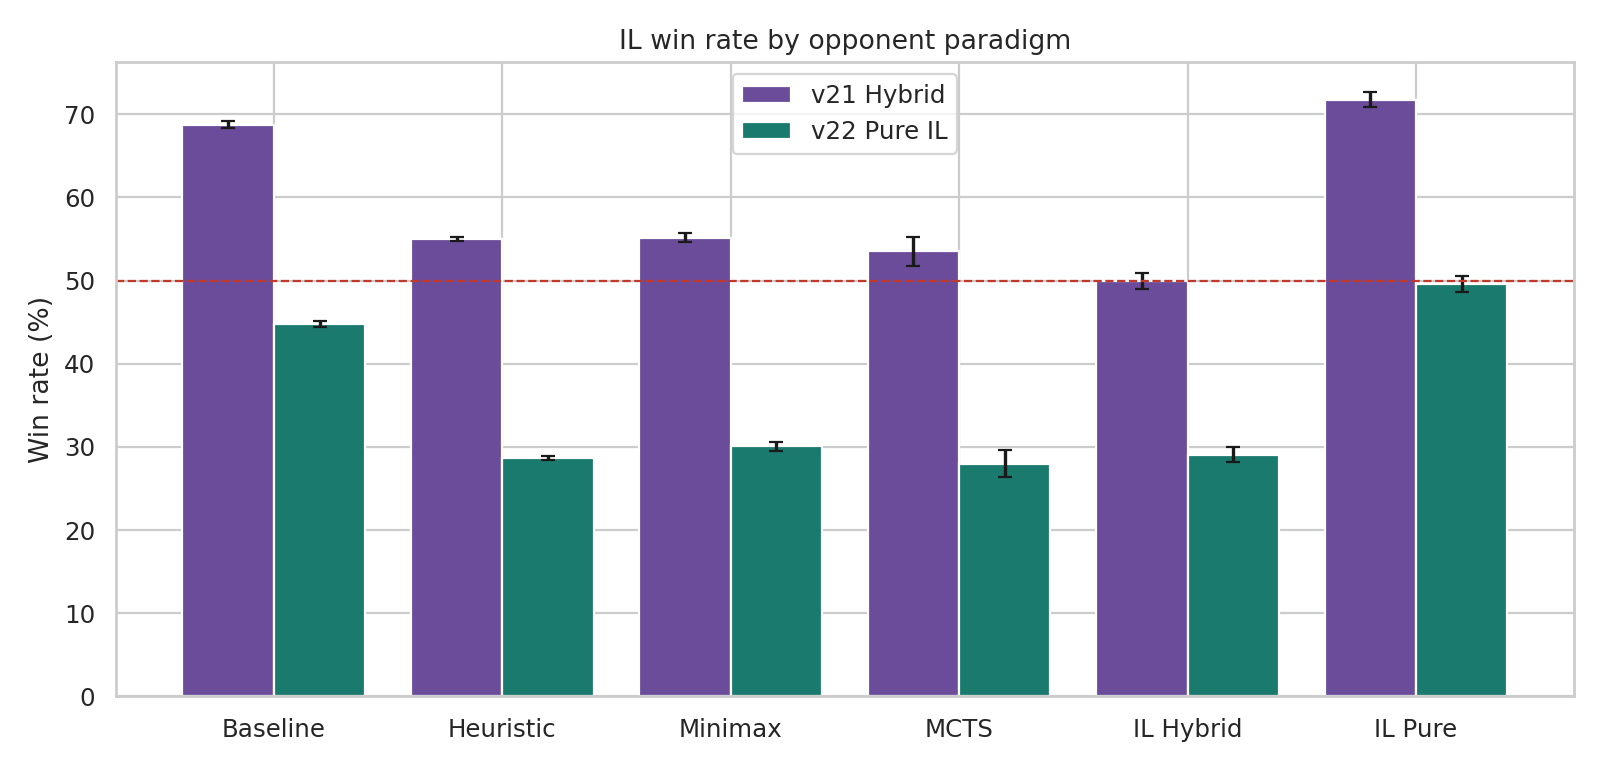
\includegraphics[width=0.92\linewidth]{images/il/il_wr_by_paradigm.png}
    \caption{Taxa de victòries dels agents d'imitació per família d'oponent. \texttt{v21} supera \texttt{v22} en els sis blocs, amb diferències d'aproximadament 20--26~pp.}
    \label{fig:il_paradigm}
\end{figure}

\begin{figure}[htbp]
    \centering
    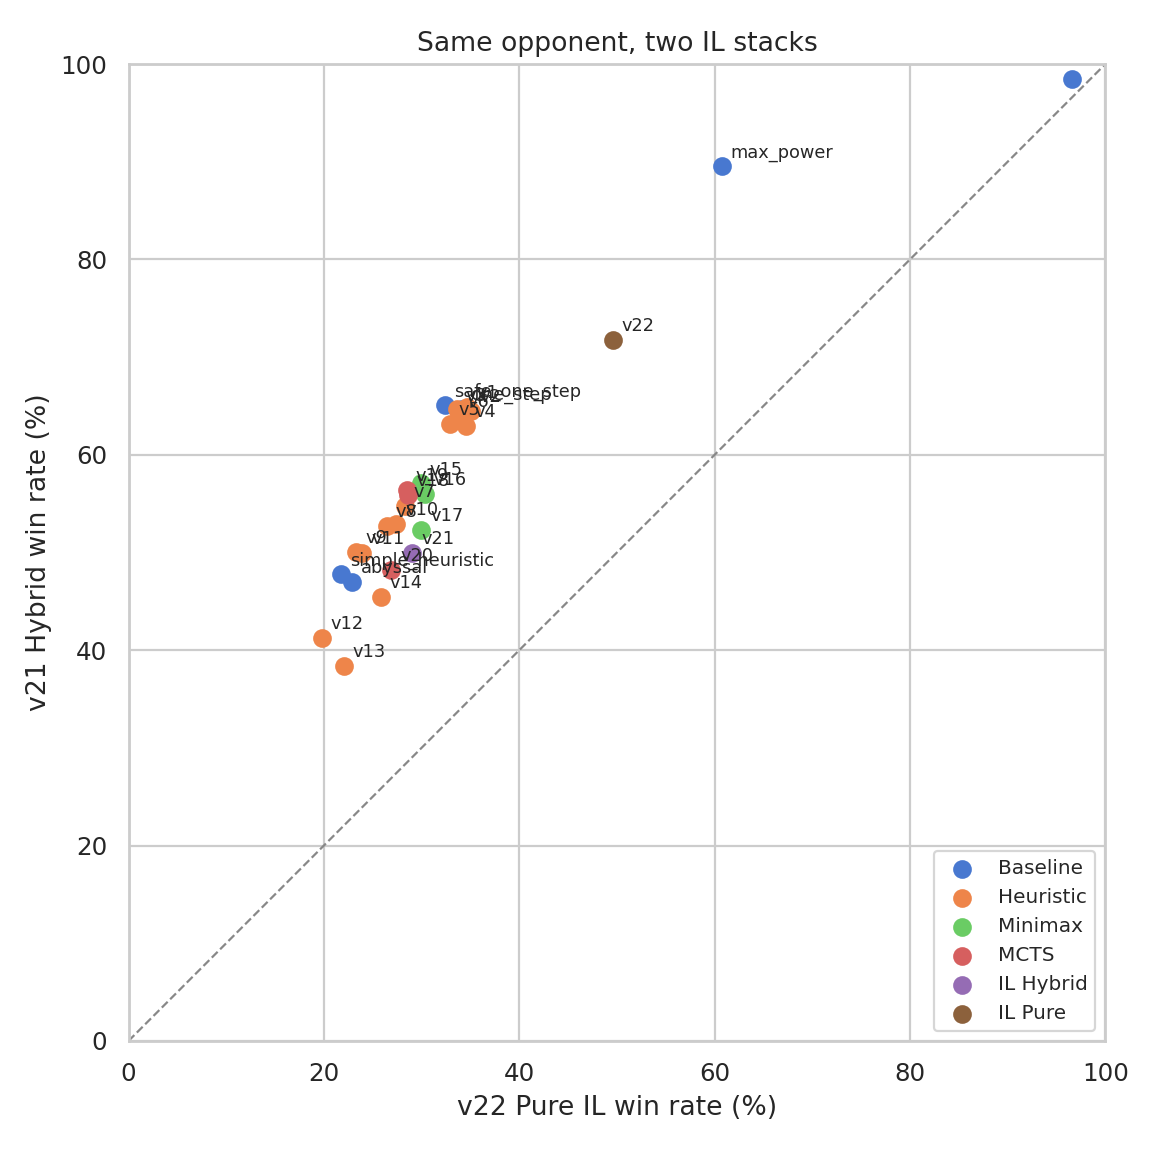
\includegraphics[width=0.85\linewidth]{images/il/il_wr_scatter.png}
    \caption{Taxa de victòries de \texttt{v21} i \texttt{v22} per oponent. Tots els punts queden \emph{per sobre} de la diagonal $y=x$: \texttt{v21} obté el valor superior en 28 de 28 enfrontaments. La diferència màxima és de 32,6~pp contra \texttt{safe\_one\_step}.}
    \label{fig:il_scatter}
\end{figure}

% ============================================================
\FloatBarrier
\section{Comparació entre els cinc paradigmes}
\label{sec:res_cross}

\begin{table}[H]
\centering
\caption{Síntesi dels cinc paradigmes amb \texttt{v12} com a comparador comú. Les variants són les que obtenen el millor resultat observat dins de cada família; aquesta selecció és posterior a l'experiment. L'MCTS té una mostra menor i el PPO no participa en la matriu completa.}
\label{tab:paradigm_summary}
\small
\begin{tabularx}{\textwidth}{llrrX}
\toprule
\textbf{Paradigma} & \textbf{Variant} & \textbf{$n$} & \textbf{vs \texttt{v12}} & \textbf{Lectura} \\
\midrule
Heurístiques & \texttt{v12} & 10.000 & 50,1\% & Autojoc de referència; 59,91\% contra Abyssal. \\
Minimax d'un torn & \texttt{v17} & 10.000 & 40,94\% & El prior cap a \texttt{v14} millora les altres variants, però no supera \texttt{v12}. \\
MCTS ras & \texttt{v20} & 1.000 & 42,7\% & PUCT redueix la discrepància amb \texttt{v14}; marge aproximat de $\pm 3$~pp. \\
Imitació & \texttt{v21} & 10.000 & 41,28\% & El model decideix quan canviar i \texttt{v14} executa l'acció. \\
PPO & model A & 10.000 & 34,1\% & Experiment separat, inicialitzat per clonatge de \texttt{v8}. \\
\bottomrule
\end{tabularx}
\end{table}


La Taula~\ref{tab:paradigm_summary}, juntament amb la Taula~\ref{tab:overall_wr} i la Taula~\ref{tab:vs_disc}, utilitzen comparadors comuns per contrastar els cinc paradigmes. És la comparació més directa disponible per als cinc paradigmes, però no iguala el pressupost de l'MCTS, no controla el cost d'entrenament i selecciona posteriorment la variant amb millor resultat de cada família. Sota aquestes condicions, cap de les implementacions de minimax, MCTS, imitació o PPO arriba al 50\% contra \texttt{v12}.

\begin{table}[H]
\centering
\caption{Taxa de victòries global com a \emph{nosaltres} contra els 28 oponents. Heurístiques, minimax i IL: $253.000$ partides (25 oponents $\times 10.000$ + 3 MCTS $\times 1.000$). MCTS: $28.000$ partides, totes les cel·les amb $n=1.000$. No es poden comparar els dos globals com si tinguessin la mateixa precisió; per ordenar \texttt{v20} contra \texttt{v17} cal mirar cel·les de matchup. Font: \texttt{data/benchmarks/all\_10k/gen9randombattle}.}
\label{tab:overall_wr}
\small
\begin{tabular}{rlrrl}
\toprule
\textbf{Rang} & \textbf{Agent} & \textbf{Partides} & \textbf{WR (\%)} & \textbf{Paradigma} \\
\midrule
1  & \texttt{v12}              & 253.000 & 69,01 & Heurística \\
2  & \texttt{v13}              & 253.000 & 67,63 & Heurística \\
3  & \texttt{v14}              & 253.000 & 62,03 & Heurística \\
4  & \texttt{abyssal}          & 253.000 & 62,00 & Baseline \\
5  & \texttt{simple\_heuristic}& 253.000 & 61,93 & Baseline \\
6  & \texttt{v20}              &  28.000 & 59,66 & MCTS (cel·les $n=1$k) \\
7  & \texttt{v11}              & 253.000 & 59,26 & Heurística \\
8  & \texttt{v9}               & 253.000 & 58,86 & Heurística \\
9  & \texttt{v21}              & 253.000 & 58,71 & IL híbrid \\
10 & \texttt{v17}              & 253.000 & 57,89 & Minimax \\
11 & \texttt{v10}              & 253.000 & 55,66 & Heurística \\
12 & \texttt{v8}               & 253.000 & 55,43 & Heurística \\
13 & \texttt{v16}              & 253.000 & 54,30 & Minimax \\
14 & \texttt{v7}               & 253.000 & 54,25 & Heurística \\
15 & \texttt{v18}              &  28.000 & 54,02 & MCTS (cel·les $n=1$k) \\
16 & \texttt{v15}              & 253.000 & 53,80 & Minimax \\
17 & \texttt{v19}              &  28.000 & 53,29 & MCTS (cel·les $n=1$k) \\
\midrule
-- & \texttt{v5}               & 253.000 & 45,86 & Heurística (altiplà) \\
-- & \texttt{v1}               & 253.000 & 44,25 & Heurística (altiplà) \\
-- & \texttt{v22}              & 253.000 & 33,49 & IL pur \\
-- & \texttt{max\_power}       & 253.000 & 19,66 & Baseline \\
-- & \texttt{random}           & 253.000 &  4,20 & Baseline (àncora Elo $=1000$) \\
\bottomrule
\end{tabular}
\end{table}


\begin{table}[H]
\centering
\caption{Enfrontaments de referència. Les files amb MCTS tenen $n=1.000$ i la resta, $n=10.000$. \texttt{v12} contra Abyssal (59,91\% $\pm 0,96$~pp) és el principal resultat contra un agent extern basat en regles.}
\label{tab:vs_disc}
\small
\begin{tabular}{lrrrr}
\toprule
\textbf{Agent} & \textbf{vs Abyssal} & \textbf{vs \texttt{v12}} & \textbf{vs \texttt{v14}} & \textbf{vs SimpleH} \\
\midrule
\texttt{v12} & 59,91 & 50,1 (autojoc) & 56,01 & 59,75 \\
\texttt{v13} & 55,34 & 48,85 & 57,71 & 56,10 \\
\texttt{v14} & 51,36 & 44,74 & 50,1 (autojoc) & 50,66 \\
\texttt{v20} ($n=1$k) & 49,0 & 42,7 & 47,0 & 49,2 \\
\texttt{v21} & 46,98 & 41,28 & 45,43 & 47,76 \\
\texttt{v17} & 46,79 & 40,94 & 43,61 & 46,75 \\
\texttt{v16} & 41,86 & 35,92 & 39,56 & 40,65 \\
\texttt{v15} & 41,72 & 36,04 & 39,43 & 41,23 \\
\texttt{v18} ($n=1$k) & 42,2 & 34,0 & 40,0 & 42,0 \\
\texttt{v1}  & 30,64 & 23,29 & 32,09 & 30,26 \\
\texttt{v22} & 22,90 & 19,80 & 25,81 & 21,73 \\
\bottomrule
\end{tabular}
\end{table}


\begin{figure}[htbp]
    \centering
    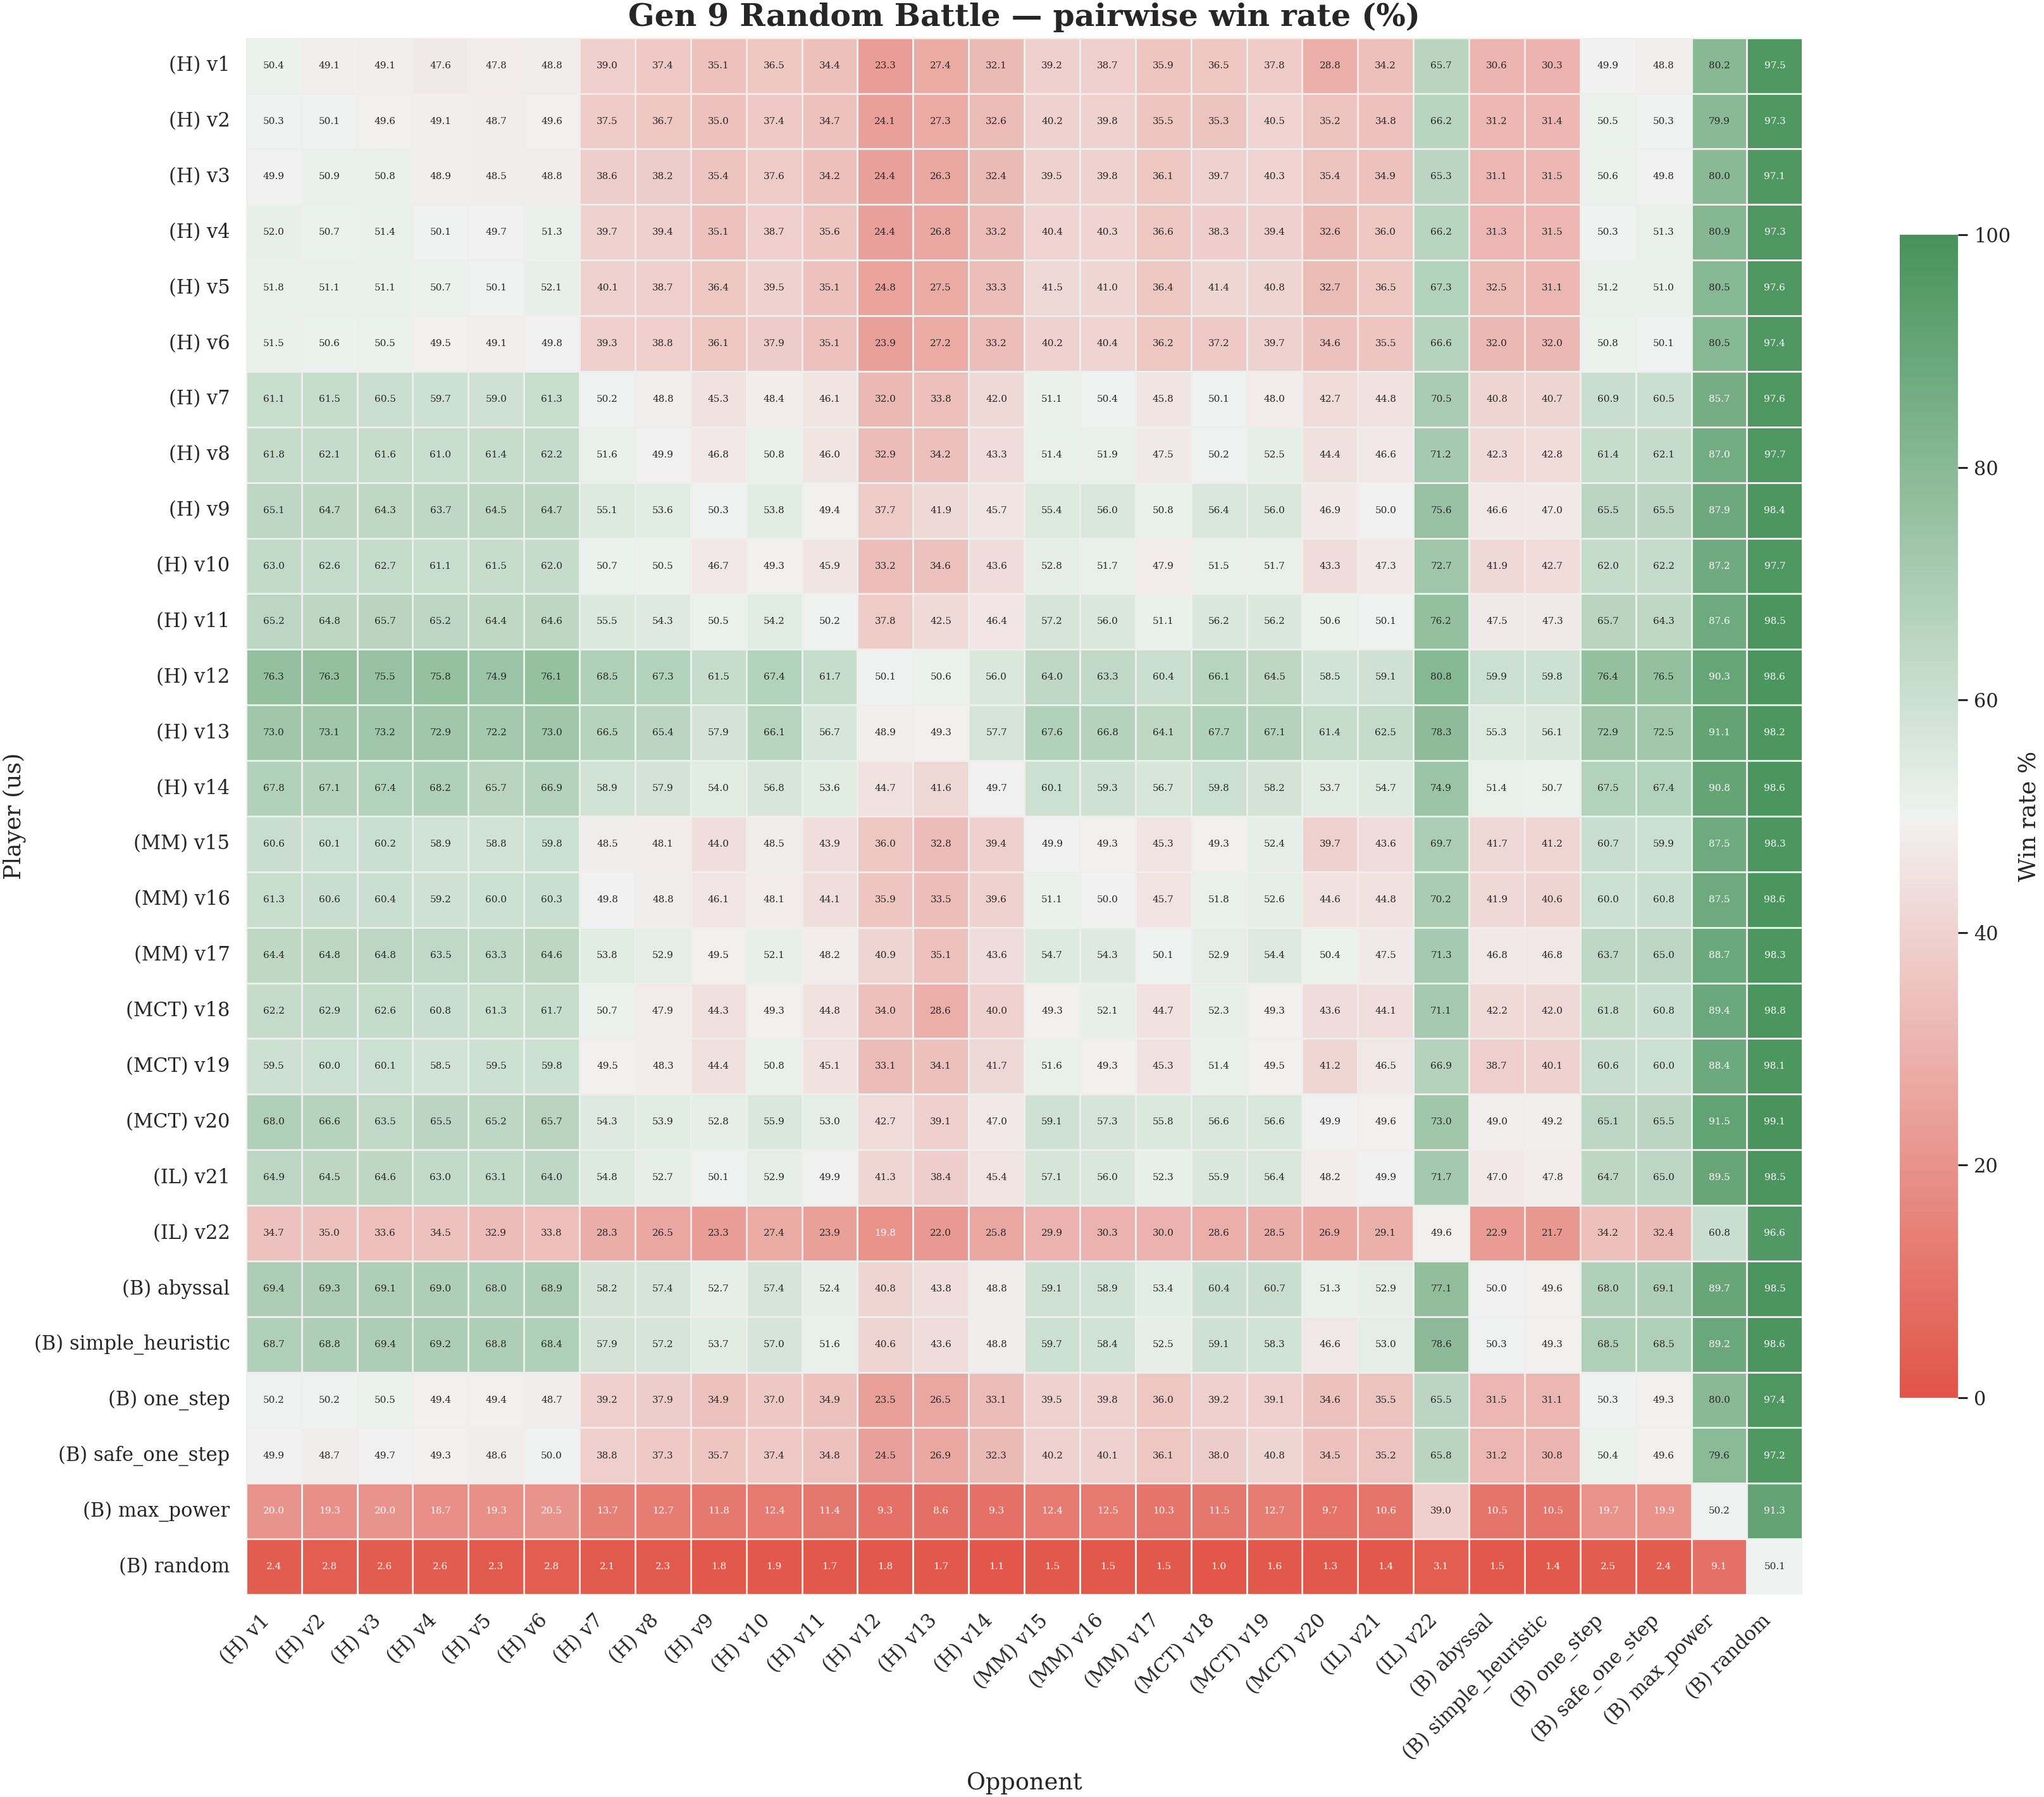
\includegraphics[width=\linewidth]{images/results/gen9_winrate_heatmap.png}
    \caption{Mapa de calor de la taxa de victòries a \texttt{gen9randombattle}. La fila és l'agent analitzat i la columna, l'oponent. Prefixos: (H) heurística, (MM) minimax, (MCT) MCTS, (IL) imitació i (B) agent de referència. Les cel·les amb MCTS tenen $n=1.000$; la resta, $n=10.000$.}
    \label{fig:heatmap}
\end{figure}

\subsection{Abyssal com a agent de referència}

Fins a \texttt{v12}, cap heurística interna supera el 50\% contra Abyssal. \texttt{v7}--\texttt{v11} obtenen entre 41\% i 48\%; \texttt{v12} arriba a 59,91\%. \texttt{v14} obté 51,36\%, \texttt{v21} 46,98\%, \texttt{v20} 49,0\% amb $n=1.000$, \texttt{v17} 46,79\% i \texttt{v22} 22,90\%. El resultat de referència és, per tant, \textbf{\texttt{v12} contra Abyssal: 59,91\% $\pm 0{,}96$~pp, $n=10.000$}.

\subsection{Escala Bradley--Terry}

Com a complement a les taxes directes de victòria per parelles, s'ajusta el model de Bradley--Terry definit a la Secció~\ref{subsec:marc_estadistic} mitjançant regressió logística per màxima versemblança (MLE) sobre la matriu completa de 784 cel·les dirigides, ancorant l'escala a $\text{Random} = 1000$ (Figura~\ref{fig:elo_bars}). Aquesta representació condensa les preferències relatives empíriques en una dimensió latent contínua de força competitiva independent de la composició del calendari d'enfrontaments.

Tal com s'observa a la Figura~\ref{fig:elo_bars}, \texttt{v12} (1812) i \texttt{v13} (1802) assoleixen les puntuacions latents superiors del conjunt, corroborant la seva consistència tant davant d'adversaris d'alt nivell com davant de la resta d'heurístiques. Immediatament per sota, es produeix una convergència al voltant dels 1755 punts entre \texttt{v14} (1755), \texttt{simple\_heuristic} (1755) i Abyssal (1755). Aquesta coincidència numèrica posa de manifest un altiplà competitiu compartit: les tres polítiques basades en regles expertes assoleixen un nivell de domini equivalent sobre el conjunt del ventall, i les diferències decimals entre elles ($<0{,}3$ punts) són estadísticament negligibles.

Pel que fa a la resta de paradigmes, les seves variants més competitives s'estableixen en una franja intermèdia propera: \texttt{v20} (MCTS PUCT, 1742), \texttt{v21} (imitació híbrida XGBoost, 1729) i \texttt{v17} (minimax amb prior, 1722). A la banda inferior de l'escala, \texttt{v22} (imitació pura d'atributs sense proteccions de domini, 1529), \texttt{max\_power} (1383) i \texttt{random} (1000) delimiten la línia de base de l'entorn.

\paragraph{Precaució interpretativa: per què no constitueix una classificació unificada.}
Convé subratllar amb rigor que la Figura~\ref{fig:elo_bars} reflecteix una estimació global de força latent sobre la matriu observada i \textbf{no s'ha d'interpretar com una classificació lineal o un rànquing ordinal absolut}. Aquesta distinció és crítica per tres raons metodològiques:
\begin{enumerate}
    \item \textbf{Asimetria mostral i de pressupost en MCTS:} Mentre que els agents heurístics, minimax, imitació i referència aporten $n=10.000$ partides per cel·la (506.000 partides dirigides per agent al model), les variants d'MCTS (\texttt{v18}--\texttt{v20}) es van avaluar a $n=1.000$ per cel·la (56.000 partides) i sota un pressupost d'inferència estrictament acotat a 5 torns de desplegament. Aquesta diferència de volum mostral implica una variància d'estimació superior que desaconsella intercalar ordinalment MCTS amb la resta d'agents.
    \item \textbf{Precisió asimptòtica i interpretació per estrats:} Gràcies a l'elevat volum de dades (253.000 partides com a fila i el mateix volum com a oponent, 506.000 aparicions per a cada agent no MCTS), l'error estàndard asimptòtic de les estimacions de màxima versemblança és extremadament reduït ($\pm 2$--$3$ punts Elo), fent que la separació entre grans macroestrats (com els 1812 de \texttt{v12} enfront dels 1755 de \texttt{v14}) sigui estadísticament inequívoca. No obstant això, aquesta precisió global no autoritza a proclamar superioritat ordinal \emph{dins} d'un mateix altiplà (com les diferències decimals entre \texttt{v14}, Abyssal i \texttt{simple\_heuristic} a 1755 punts). Per a aquestes comparacions de detall, el treball recorre als intervals de confiança de Wilson al $95\%$ ($\pm 0{,}96$~pp) sobre les taxes directes de victòria per parelles.
    \item \textbf{Intransitivitat i dinàmiques de tipus (pedra-paper-tisores):} Tal com evidencia el mapa de calor dirigit (Figura~\ref{fig:heatmap}) i la inversió d'estils de la Secció~\ref{sec:res_inversion}, l'espai de joc de Pokémon Random Battles presenta cicles intransitius d'especialització que cap projecció unidimensional pot capturar íntegrament sense pèrdua d'informació estructural.
\end{enumerate}
Per aquest motiu, l'anàlisi comparativa interparadigma s'articula fonamentalment a través de l'oponent comú \texttt{v12} (Taula~\ref{tab:paradigm_summary}) i de les taxes agrupades per família (Taula~\ref{tab:overall_wr}), evitant tractar la matriu heterogènia com una lliga única.

\begin{figure}[htbp]
    \centering
    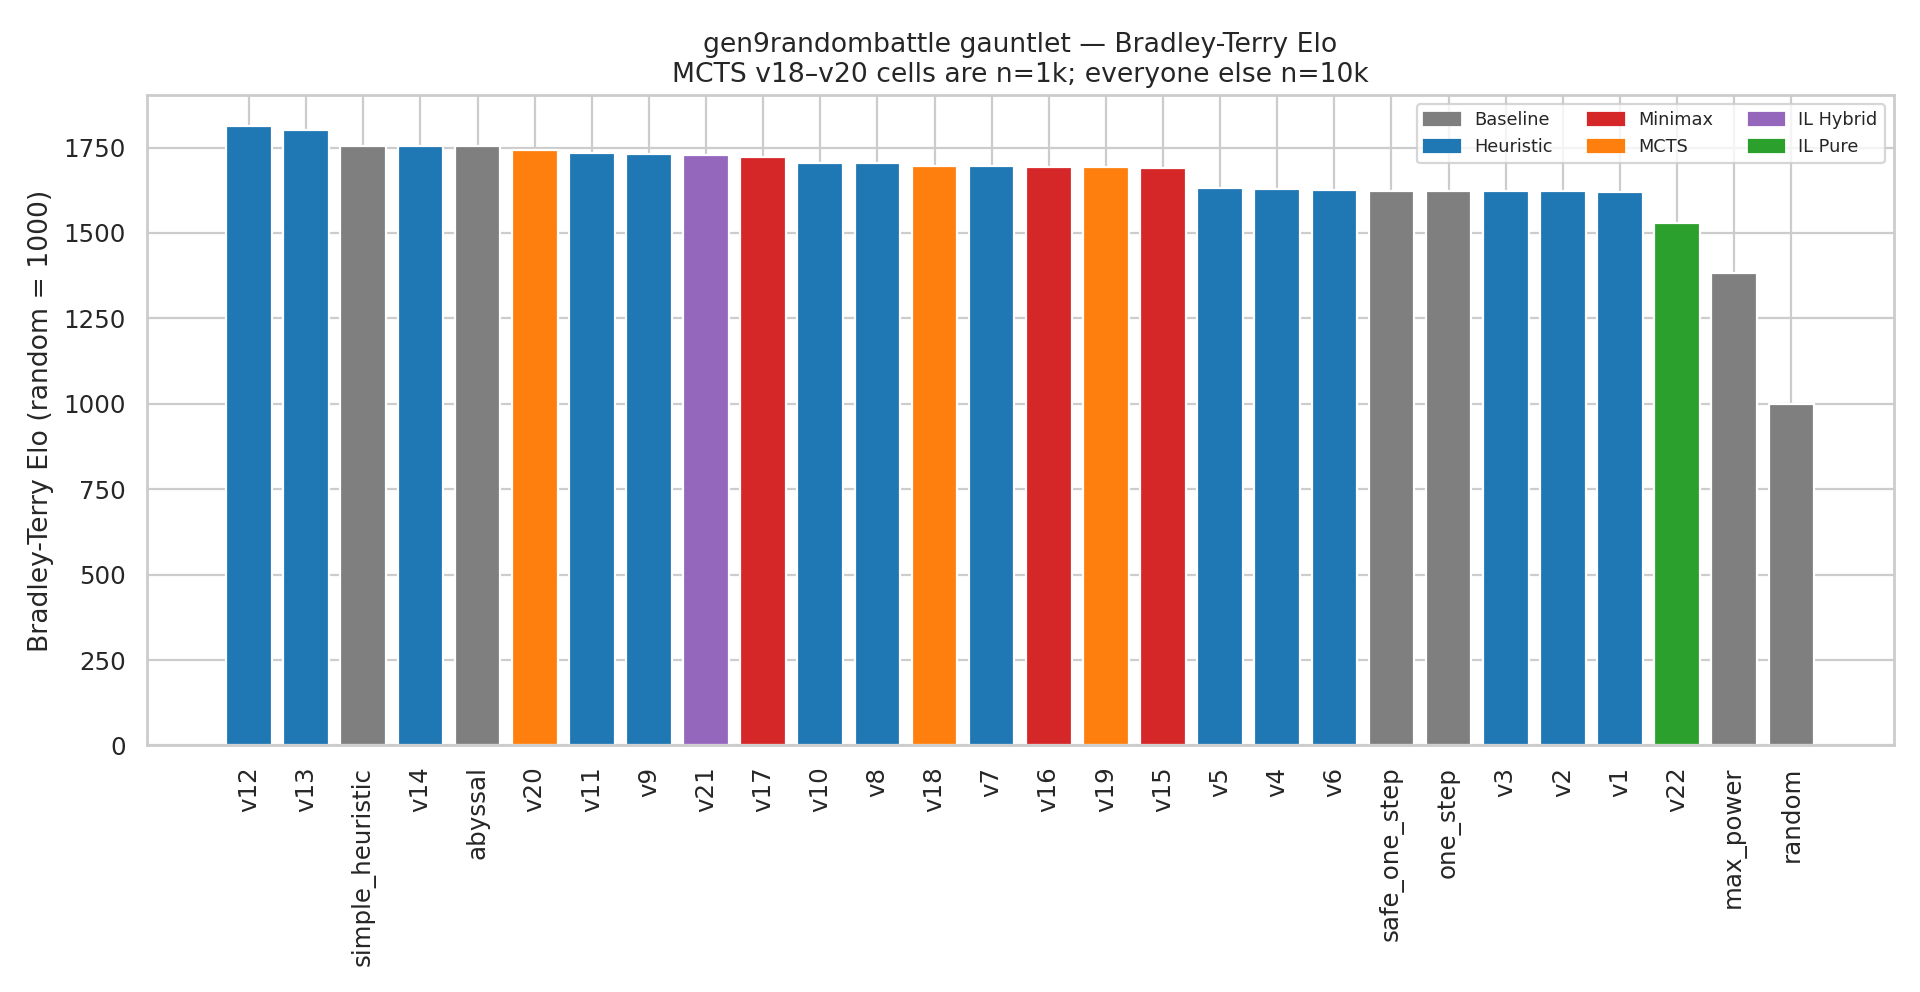
\includegraphics[width=0.92\linewidth]{images/results/gen9_elo_bars.png}
    \caption{Escala latent Bradley--Terry ancorada a \texttt{random}${}=1000$ ajustada sobre les dues orientacions de la matriu. \texttt{v12} i \texttt{v13} obtenen les puntuacions més altes; \texttt{v14}, Abyssal i Simple Heuristic comparteixen un altiplà a 1755 punts. Les files i columnes d'MCTS aporten una desena part de partides al model ($n=1.000$).}
    \label{fig:elo_bars}
\end{figure}

% ============================================================
\FloatBarrier
\section{Classificació pública: avaluació exploratòria de \texttt{v14}}
\label{sec:res_ladder}

\begin{table}[H]
\centering
\caption{Ladder pública de \texttt{v14} contra humans (\texttt{gen9randombattle}, usuari \texttt{SirPThesis}, 9--10 de juny de 2026). Font: \texttt{data/testing/logs/logs\_v14\_online/battle\_history.csv}. El snapshot del pla de juny (98 partides, 40,8\%, Elo $\sim$1151) és un \emph{prefix} d'aquest mateix log, pres a prop del pic d'Elo: no és la mostra final.}
\label{tab:ladder_v14}
\small
\begin{tabular}{lr}
\toprule
\textbf{Mètrica} & \textbf{Valor} \\
\midrule
Partides úniques acabades & 431 \\
Victòries & 170 / 431 \\
WR en brut & 39,44\% $\pm 4{,}6$~pp \\
Només torns $\ge 10$ (taules tàctiques) & 35,43\% ($n=398$) \\
Partides curtes (torns $<10$) & 33 (sobretot abandons; inflen el WR brut) \\
Elo & $1085 \rightarrow 1038$ (rang $1000$--$1263$) \\
Errors / fallbacks & 0 / 13 \\
Finestra & 2026-06-09 21:54 -- 2026-06-10 18:32 \\
\bottomrule
\end{tabular}
\end{table}


A la classificació pública oficial (\emph{ladder}), \texttt{v14} va disputar 431 partides entre el 9 i el 10 de juny de 2026, assolint una taxa global del 39,44\% $\pm 4,6$~pp (Taula~\ref{tab:ladder_v14} i Figura~\ref{fig:ladder_wr}).

\begin{figure}[htbp]
    \centering
    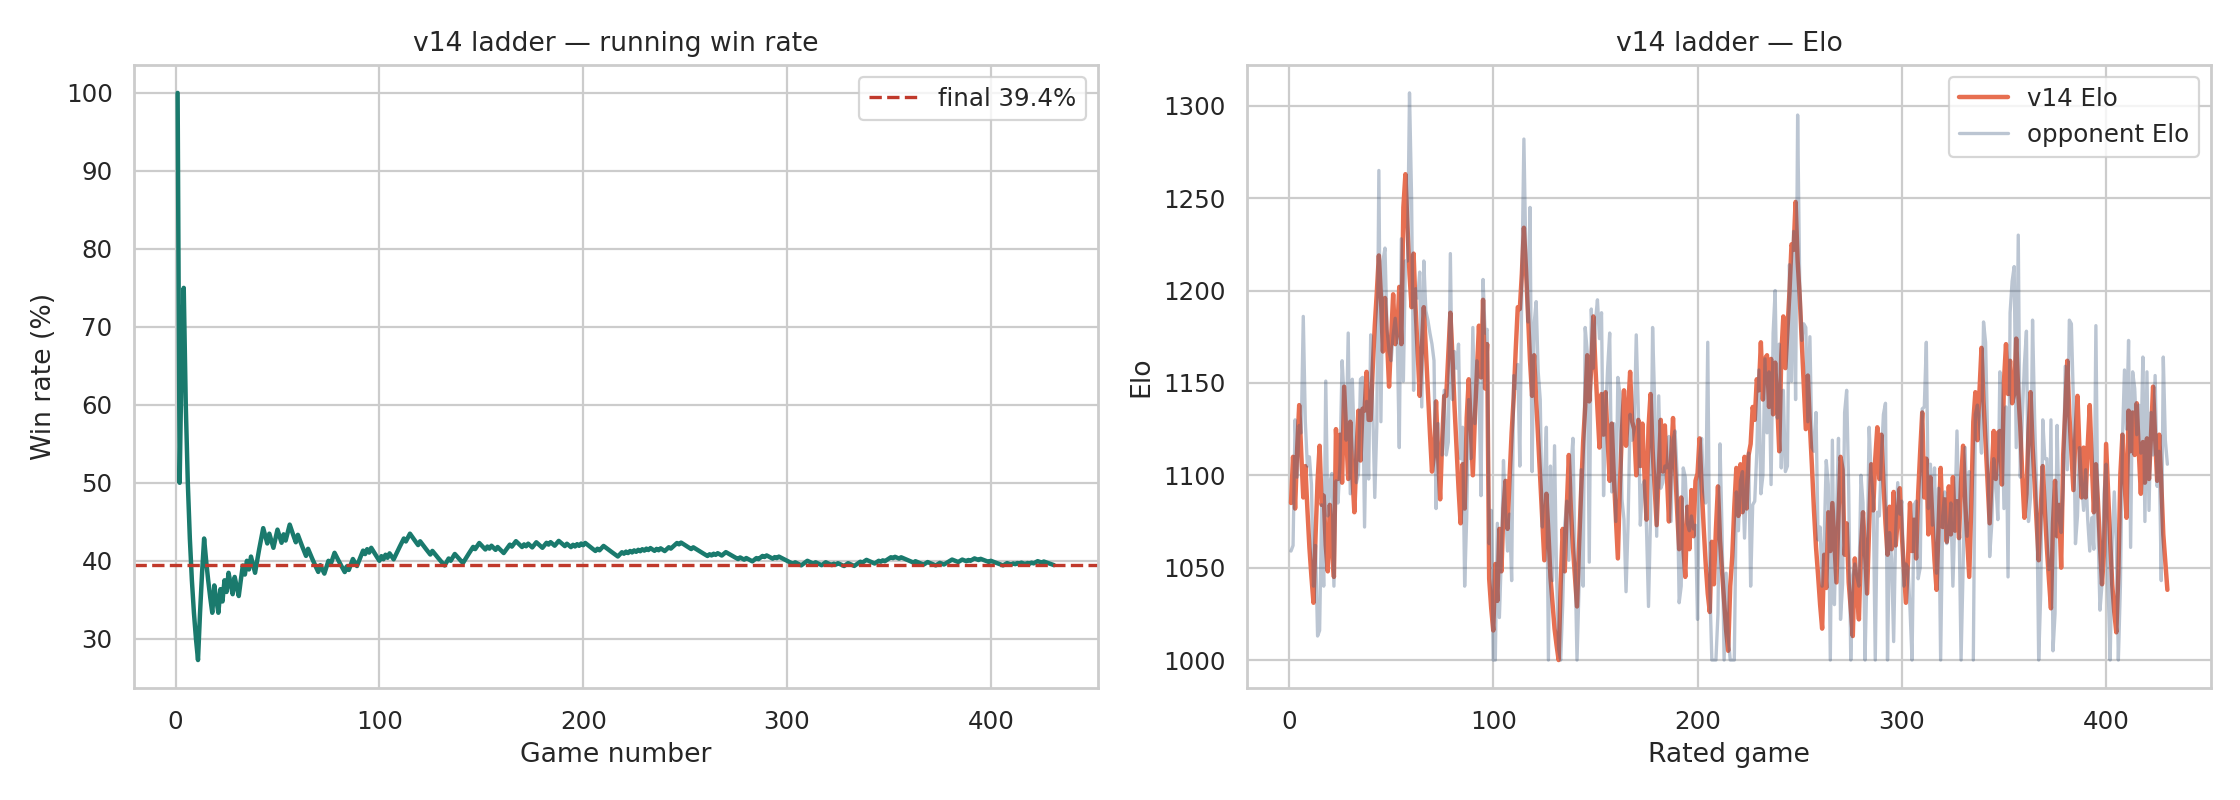
\includegraphics[width=0.92\linewidth]{images/results/ladder_wr_elo.png}
    \caption{Taxa de victòries acumulada i Elo de \texttt{v14} a la classificació pública: 431 partides entre el 9 i el 10 de juny de 2026, 39,44\% $\pm 4,6$~pp i Elo de 1085 a 1038 (màxim 1263). Una instantània prefixa de 98 partides, presa prop del màxim d'Elo, no representa el resultat final.}
    \label{fig:ladder_wr}
\end{figure}

\begin{figure}[htbp]
    \centering
    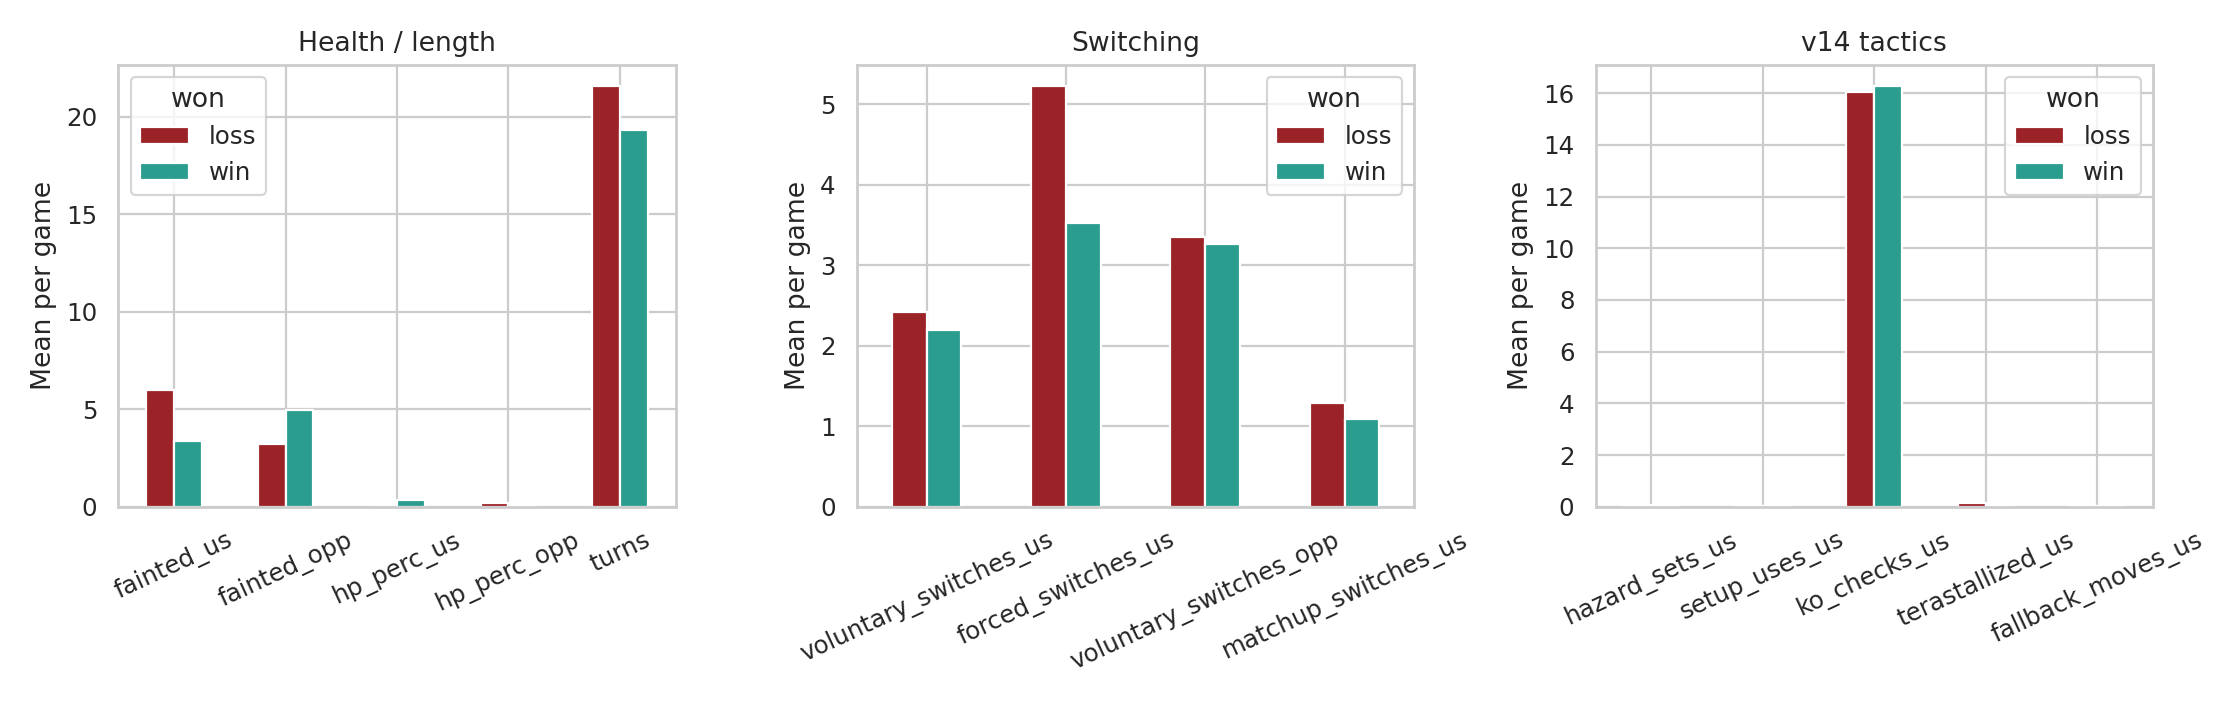
\includegraphics[width=0.92\linewidth]{images/results/ladder_win_vs_loss.png}
    \caption{Telemetria de \texttt{v14} al \emph{ladder}, separada per victòria i derrota: durada i membres debilitats, canvis, i tàctiques (\texttt{ko\_checks} $\sim$16 per partida; preparació, perills i Teracristal·lització molt baixos). El perfil tàctic s'assembla al de la matriu local.}
    \label{fig:ladder_wl}
\end{figure}

En les partides d'almenys 10 torns, \texttt{v14} utilitza la Teracristal·lització en 45 de 398 combats i obté un 20\% de victòries en aquest subconjunt. La telemetria comparativa entre victòries i derrotes (Figura~\ref{fig:ladder_wl}) mostra que presenta moltes comprovacions de debilitament i pocs moviments de preparació, un perfil semblant al de la matriu local. Com que la durada és posterior a les decisions i està relacionada amb el resultat, la taxa filtrada no s'interpreta com una estimació alternativa de rendiment.

Aquesta avaluació pública té un caràcter \textbf{exploratori i anecdòtic}: demostra que el sistema funciona i és capaç de competir en un entorn real amb jugadors humans, però no constitueix una validació estadísticament rigorosa. Amb només 431 partides i una taxa de desconnexions significativa, la mostra és insuficient per a una estimació d'Elo estable. A més, la complexitat matemàtica del domini ---equips aleatoris amb centenars de variables ocultes, com s'ha formalitzat als Capítols~\ref{chap:marc_teoric} i~\ref{chap:metodologia}--- exigeix un volum de partides molt superior per obtenir intervals de confiança acceptables contra oponents no controlats. La selecció d'oponents no està controlada i la mostra no permet inferir el rendiment que hauria obtingut \texttt{v12}.

% ============================================================
\FloatBarrier
\section{PPO contra \texttt{v12}}
\label{sec:res_ppo}

El cinquè paradigma s'avalua fora de la matriu, contra \texttt{v12}, amb $n=10.000$ i les dues orientacions (Secció~\ref{sec:disseny_experiments}). L'entorn, la màscara \texttt{Discrete(14)}, el vector de 328 dimensions i el clonatge de \texttt{v8} (400 partides) són els del Capítol~\ref{chap:implementacio}. Aquí es llegeixen les validacions congelades i el model A.

\begin{table}[htbp]
\centering
\caption{Currículum i avaluacions de MaskablePPO. Els artefactes i hiperparàmetres d'entrenament es detallen a la Taula~\ref{tab:ppo_curriculum_impl}. El resultat principal correspon al model A contra \texttt{HeuristicV12} ($n=10.000$ i ambdues orientacions). La fase~4 només informa de la taxa interna durant l'entrenament, no d'una avaluació independent.}
\label{tab:ppo_head}
\label{tab:ppo_curriculum_eval}
\small
\renewcommand{\arraystretch}{1.15}
\begin{tabularx}{\textwidth}{llrrl>{\raggedright\arraybackslash}X}
\toprule
\textbf{Fase} & \textbf{Oponent} & \textbf{$n$} & \textbf{TV (\%)} & \textbf{Porta de pas} & \textbf{Estat / Observacions} \\
\midrule
1 & Random & 1.000 & 91,8 & $\ge 90\%$ & Superada (graduació) \\
1.5 & MaxBP & 1.000 & 70,5 & $>70\%$ & Superada per estimació puntual \\
2 & \texttt{v8} & 1.000 & 40,6 & $>55\%$ & No superada \\
\textbf{3 (resultat)} & \textbf{\texttt{v12}} & \textbf{10.000} & \textbf{34,1} & --- & Mesura final model A (328 dims, $\pm 0{,}93$~pp) \\
3B (diagnòstic) & \texttt{v12} & 1.000 & 32,6 & --- & Model B, taxa $1{,}5\times10^{-4}$ \\
4 (interrompuda) & \texttt{v12} & 12.554 & 33,5 & --- & Taxa d'entrenament (346 dims, clonatge \texttt{v14}) \\
Control & Random & 1.000 & 98,3 & --- & Verificació d'accions legals (model A) \\
Matriu (context) & \texttt{v8} vs \texttt{v12} & 10.000 & 32,9 & --- & Rendiment del professor de clonatge \\
\bottomrule
\end{tabularx}
\end{table}


\subsection{Resultat principal}

Per avaluar la robustesa del resultat, es van executar \textbf{5 entrenaments independents} amb llavors aleatòries diferents, mantenint la mateixa arquitectura, observació i currículum. El model A (\texttt{p3\_v12\_lr5e5\_flat.zip}) és representatiu del rendiment mitjà del conjunt.

La taxa de victòries mitjana de les 5 execucions contra \texttt{HeuristicV12} és:

\begin{center}
\textbf{34,1\%} \quad $\pm 0{,}93$~pp \quad (IC $\sim$33,2--35,0\%), \quad $\bar{x} = 34{,}1\%$, $\sigma = 0{,}7$~pp.
\end{center}

Les cinc llavors obtenen taxes entre 33,2\% i 34,9\%, confirmant l'estabilitat del resultat. Per orientació, el model A obté 34,2\% (1709/5000) com a p1 i 33,9\% (1696/5000) com a p2, amb 17,2 torns de mitjana. En el control contra Random, la mitjana de les 5 execucions és de \textbf{98,3\%} amb $n=1.000$. Això confirma que la política produeix accions legals i eficaces contra un agent aleatori, però cap de les cinc execucions no arriba al 50\% contra \texttt{v12}.

A la matriu, \texttt{v8} obté \textbf{32,9\%} contra \texttt{v12} ($n=10.000$). La diferència puntual respecte de la mitjana PPO és d'1,2~pp i els intervals se superposen en totes cinc llavors; per tant, no hi ha evidència clara que el model final superi el seu professor de clonatge en aquest comparador.

\subsection{Currículum}

La Taula~\ref{tab:ppo_head} i la Figura~\ref{fig:ppo_curriculum_curves} separen artefactes d'entrenament (Capítol~\ref{chap:implementacio}) i validació congelada. Les dues primeres etapes compleixen el criteri operatiu; la fase~2 no, i la fase~3 s'executa com a prova de continuació.

No és correcte descriure el currículum com quatre graduacions reeixides. Una configuració amb taxa $1{,}5\times 10^{-4}$ i 16 entorns obté 32,6\% contra \texttt{v12} amb $n=1.000$. L'extensió a 346 dimensions, inicialitzada amb \texttt{v14}, es va interrompre amb una taxa d'entrenament aproximada del 33,5\%. Aquests valors són diagnòstics i no substitueixen l'avaluació del model A.

\subsection{Interpretació del límit observat}

Hi ha diverses explicacions compatibles amb el 34,1\%, però les dades no permeten triar-ne una de manera causal:

\begin{enumerate}
    \item \textbf{Professor inicial.} El clonatge parteix de \texttt{v8}, que obté 32,9\% contra \texttt{v12}. El resultat final és proper a aquest punt de partida.
    \item \textbf{Salt de dificultat.} La política no arriba a paritat amb \texttt{v8} abans de passar a \texttt{v12}; per tant, la fase següent comença sense haver consolidat l'anterior.
    \item \textbf{Observació sense memòria.} El vector resumeix l'estat actual, però la política no és recurrent i pot perdre informació temporal útil sobre moviments revelats o patrons del rival.
    \item \textbf{Recompensa modelada.} HP, debilitaments, modificadors i perills proporcionen senyal dens, però poden premiar estats intermedis que no maximitzen la victòria final.
    \item \textbf{Variabilitat d'entrenament.} Les cinc llavors independents mostren una desviació estàndard de 0,7~pp, cosa que suggereix que el límit observat és robust a la inicialització, però no descarta que una configuració d'hiperparàmetres diferent obtingui un resultat substancialment millor.
\end{enumerate}

Amb aquesta observació, recompensa, inicialització i pressupost, cap de les cinc execucions de MaskablePPO no supera \texttt{v12}. La conclusió es limita al sistema executat, no a PPO en general. El resultat més informatiu és que vèncer Random no prediu l'èxit contra una heurística amb coneixement de posició i mecàniques de format.

% ============================================================
\FloatBarrier
\section{Discussió}
\label{sec:res_disc}

\subsection{Patró d'integració residual}

\texttt{v21} (imitació), \texttt{v17} (minimax) i \texttt{v20} (MCTS) comparteixen un patró: conserven les regles tàctiques de \texttt{v14} i hi afegeixen un mòdul que intervé en una fracció de les decisions (Taula~\ref{tab:residual_integration}). Dins de cada família, aquestes variants obtenen un resultat superior a les alternatives que substitueixen més sovint la proposta de \texttt{v14}. PPO, en canvi, no hereta l'executor \texttt{v14} i queda al nivell del professor \texttt{v8}.

\begin{table}[htbp]
    \centering
    \caption{Integració residual sobre \texttt{v14}. El percentatge de torns és la fracció en què s'executa el mòdul afegit; la discrepància és la taxa en què aquest mòdul no retorna l'acció de \texttt{v14} (no aplica a XGBoost ni a PPO). $n=10.000$ tret de \texttt{v20} ($n=1.000$).}
    \label{tab:residual_integration}
    \small
    \renewcommand{\arraystretch}{1.2}
    \begin{tabularx}{\textwidth}{lXccc}
        \toprule
        \textbf{Variant} & \textbf{Mòdul} & \textbf{Torns} & \textbf{Discrepància} & \textbf{vs \texttt{v12}} \\
        \midrule
        \texttt{v17} & maximin d'un torn & 16,3\% & 36,6\% & 40,94\% \\
        \arrayrulecolor{gray!30}\hline\arrayrulecolor{black}
        \texttt{v20} & PUCT, prior $0{,}70$ & 15,5\% & 18,7\% & 42,7\% \\
        \arrayrulecolor{gray!30}\hline\arrayrulecolor{black}
        \texttt{v21} & XGBoost atacar/canviar & 15\% & --- & 41,28\% \\
        \arrayrulecolor{gray!30}\hline\arrayrulecolor{black}
        PPO A & política neuronal & 100\% & --- & 34,1\% \\
        \bottomrule
    \end{tabularx}
\end{table}

El patró no demostra que qualsevol arquitectura híbrida sigui superior. Les variants difereixen en més d'un component i s'han seleccionat després d'observar els resultats. Sí que aporta evidència consistent que, amb les representacions i pressupostos implementats, preservar restriccions tàctiques de domini és important.

\subsection{Resposta conjunta a la pregunta de recerca}

\begin{enumerate}
    \item La seqüència heurística mostra increments associats a posició, control del ritme i mecàniques de Generació~IX. \texttt{v12} obté el millor resultat observat ($69{,}01\%$). El contrast amb \texttt{v13} ---mateixa selecció de substitut, Teracristal·lització reduïda un 79\%--- només retrocedeix $\approx 1{,}4$~pp ($67{,}63\%$) i el duel directe no separa les dues polítiques; això suggereix, com a hipòtesi observacional, que el gruix del salt \texttt{v11}$\to$\texttt{v12} s'associa al substitut informat, no a un efecte causal aïllat de la Tera.
    \item El minimax d'un torn i l'MCTS ras no superen \texttt{v12}. Les millors variants són les que es mantenen més a prop de \texttt{v14}.
    \item El model d'imitació aporta una decisió d'alt nivell aprofitable quan \texttt{v14} executa l'acció. L'execució basada en atributs de \texttt{v22} queda clarament per sota.
    \item MaskablePPO obté 34,1\% contra \texttt{v12}, un resultat proper al de \texttt{v8} contra el mateix oponent i insuficient per afirmar una millora sobre el professor de clonatge.
    \item En el comparador comú \texttt{v12}, cap de les implementacions seleccionades de minimax, MCTS, imitació o PPO arriba al 50\%.
\end{enumerate}

\subsection{Limitacions específiques dels resultats}

\begin{itemize}
    \item Les taxes globals inclouen oponents fàcils, autojoc i etiquetes duplicades, i la ponderació difereix entre files MCTS i no MCTS.
    \item La telemetria heurística de les figures d'aquesta secció és la mitjana ponderada de la matriu completa (253.000 partides per fila); la de minimax, MCTS i imitació també cobreix tota la matriu.
    \item \texttt{endgame\_solves} de \texttt{v18} pot incloure activitat de la sonda \texttt{v14} posterior a la cerca.
    \item \texttt{LocalSim} no és el mateix motor que Showdown; un desajust de mecàniques pot introduir soroll en les simulacions.
    \item L'avaluació pública de \texttt{v14} és una mostra no controlada de 431 partides.
    \item El PPO només es compara amb \texttt{v12}; les cinc llavors confirmen l'estabilitat del resultat, però no s'ha explorat una cerca d'hiperparàmetres més àmplia.
\end{itemize}
